\section{uni2ts PackedStdScaler Patch Details}
\label{app:scaler_patch}
% ============================================================

We identified and patched an in-place tensor mutation in
\texttt{uni2ts}'s \texttt{PackedStdScaler} that silently detaches
autograd on losses depending on scaled statistics.  The issue arises
when \texttt{PackedStdScaler.transform} performs an in-place
\texttt{.copy\_()} that breaks the gradient tape.  Our patch replaces
the in-place write with a differentiable \texttt{torch.where}
operation.  \emph{All} Moirai fine-tuning results in this paper use
the patched scaler (released with our code); unpatched
\texttt{uni2ts} runs may converge differently and we have observed
silent non-convergence on \texttt{uni2ts@main}.  We recommend
upstreaming this patch to \texttt{uni2ts}.

% ============================================================
\section{Moirai Median Forecast Selection}
\label{app:moirai_median}
% ============================================================

Moirai generates probabilistic forecasts as a mixture of
distributions (StudentT, NormalFixedScale, NegativeBinomial,
LogNormal).  The heavy-tailed components (NegBin, LogNormal) produce
extreme right-tail outliers when using the \emph{mean} of forecast
samples as the point prediction; for ETTh2 at $h{=}192$, sample
means reached 21{,}431 against a target maximum of 45.5, inflating
MSE from 0.30 to 8.58.

We use the \emph{median} of 20 forecast samples as the robust point
prediction, consistent with the Moirai paper's evaluation protocol.
This eliminates sensitivity to the heavy-tailed mixture components
while preserving the distributional forecast's central tendency.

% ============================================================
\section{The Pre-Registered Prospective Test, in Full}
\label{app:prospective2}
% ============================================================

\textbf{What was registered, and when.} Predictions were written to
\texttt{results/v47\_prospective/preregistration.json} and committed to git at
a named revision before any outcome run for those cells existed; the scoring
script reads that file and the finished runs and decides nothing.
Two rules were registered against each other: the \textbf{gate rule},
gate$_\text{pre}\!\geq\!0.20 \Rightarrow$ at risk, which is the paper's own
criterion frozen while the screen still used the unfitted trend denominator, and
therefore graded on those scores rather than re-derived after seeing the outcomes; and a
\textbf{dataset rule}, dataset ${\in}$ \{ETTh1, Weather\} $\Rightarrow$
degradation, a \emph{post hoc} pattern read off the original Moirai cells and
registered as a competitor so the gate is graded against something.
Eight cells were then run (Weather, ETTm2, Electricity7, ETTh1
$\times$ Small/Base/Large, 3 seeds each) and scored by the pre-registered
outcome definition, unchanged (Table~\ref{tab:prospective}).

\textbf{Result: the outcome the gate was registered to predict never occurs.}
None of the eight cells degraded.  The gate flagged all eight, giving
\textbf{TP~0, FP~8, FN~0}: precision $0.00$, while \textbf{sensitivity and
specificity are both unestimable}: sensitivity has an empty positive class in its
denominator, and specificity is $0/8$ only because every prediction was positive.
The competing dataset rule scores no better, for the same reason.  \textbf{What
``prospective'' does and does not mean here:} the predictions were frozen before
these cells were \emph{trained}, so they are prospective with respect to the
intervention, but the datasets and their splits already existed, so this is not a
test on newly collected data.  Nor is the empty positive class an artefact of the
fitted screen: only one of the eight clears $0.20$ on either split under it
(base/ETTm2 $h{=}192$, $+0.21$ on selection windows) and it fails clause~(ii) in 0
of 3 seeds.  \textbf{Nor is the $0.20$ threshold
what fails}: re-scoring the same predictor against the same outcome at thresholds
from $0.10$ to $0.60$, moving nothing else, gives precision $0.00$ at every one,
with 8, 8, 6, 5, 3 and 2 cells flagged (Table~\ref{tab:gate_sensitivity}); the
problem is not the cutoff but that the predicted class is empty.

\textbf{What a zero-prevalence test licenses.} With no positive instance the arm
is informative in one direction only. It establishes that the gate's positive
predictions are wrong here, at every threshold swept, and that the error is not an
artefact of the operating point. It establishes \emph{nothing} about whether the
gate would detect degradation if degradation existed: that is a claim about
sensitivity, and $0/0$ is not a rate. A reader who takes this arm as a refutation
of the gate is reading past the prevalence. The regime the arm cannot reach is
one a positive control has to construct deliberately
(\S\ref{sec:exp4:poscontrol}, Appendix~\ref{app:poscontrol}), and which, on
these benchmarks, we could not construct.

% Moved here VERBATIM from the body of S7 on 21 Sep 2026, to fund the positive control's body
% paragraphs. Not reworded: two claims registered in scripts/check_paper_numbers.py match only this
% wording, and a restatement would silently drop their sites while the checker still reported clean.
\textbf{The gate does not provide a reliable ordering, and there is no actionable
threshold.}
Within Moirai ($n{=}22$ cells from six series, the only arm with enough cells to
ask), the gate's continuous score correlates \emph{negatively} with held-out
$\denc$: Spearman $\rho{=}{-}0.293$, and neither cells nor series exclude zero, so
we report the direction and not the interval (Appendix~\ref{app:clustered}).
The sign is the wrong one (higher measured pre-trained value goes with encoder
adaptation helping \emph{more}, not less, the opposite of what a preservation
heuristic needs), but the sharper point is that the magnitude is not stable:
scoring the same gate on the held-out windows instead gives $\rho{=}{-}0.518$
on the same cells.
An ordering that nearly doubles when the gate changes split is not one a
practitioner can set a threshold on, and no other quantity we measured orders
$\denc$ either (Appendix~\ref{app:predictor}).

\begin{table}[ht]
\centering
\caption{\textbf{The pre-registered prospective test.} Predictions frozen in
git before any condition-B or -D run for these cells existed. ``Degradation''
applies the paper's own definition unchanged: gate-passing $\wedge$
forg$_\text{B}{>}0$ in every seed $\wedge$ forg$_\text{D}{<}0$ in every seed.
gate$_\text{pre}$ is the frozen predictor's score, on the unfitted
denominator; gate$_\text{val}$ is the fitted selection-split gate of
\S\ref{sec:forecasting}.}
\label{tab:prospective}
% GENERATED by scripts/score_prospective.py --latex -- do not edit by hand.
\begin{center}
\footnotesize
\setlength{\tabcolsep}{4pt}
\begin{tabular}{@{}lccccc@{}}
\toprule
Cell (new) & gate$_\text{val}$ & forg$_\text{B}$ & B$-$D held-out & Degradation? & Predicted \\
\midrule
base Weather ($h{=}96$) & $+0.41$ & $-11.7$ (0/3) & $+9.4{\pm}2.0$ & no & gate\,$\times$, data\,$\times$ \\
base Weather ($h{=}192$) & $+0.59$ & $-18.1$ (0/3) & $+12.5{\pm}8.7$ & no & gate\,$\times$, data\,$\times$ \\
base ETTm2 ($h{=}96$) & $+0.30$ & $-13.1$ (0/3) & $+7.0{\pm}2.4$ & no & gate\,$\times$, data\,$\checkmark$ \\
base ETTm2 ($h{=}192$) & $+0.26$ & $-8.4$ (0/3) & $+1.3{\pm}3.4$ & no & gate\,$\times$, data\,$\checkmark$ \\
small Electricity7 ($h{=}96$) & $+0.71$ & $-16.0$ (0/3) & $-3.2{\pm}1.5$ & no & gate\,$\times$, data\,$\checkmark$ \\
small Electricity7 ($h{=}192$) & $+0.76$ & $-18.6$ (0/3) & $-2.6{\pm}2.1$ & no & gate\,$\times$, data\,$\checkmark$ \\
large ETTh1 ($h{=}96$) & $+0.35$ & $+14.1$ (3/3) & $+28.2{\pm}4.9$ & \textbf{yes} & gate\,$\checkmark$, data\,$\checkmark$ \\
large Weather ($h{=}96$) & $+0.47$ & $+7.9$ (3/3) & $+12.0{\pm}7.5$ & \textbf{yes} & gate\,$\checkmark$, data\,$\checkmark$ \\
\bottomrule
\end{tabular}
\end{center}

\end{table}

\begin{table}[ht]
\centering
\caption{Gate threshold sensitivity on the eight pre-registered cells
(\S\ref{sec:analysis:prospective}). The predictor and the outcome definition
are both as pre-registered; only the threshold moves. Bold is the operating
point used in the paper.}
\label{tab:gate_sensitivity}
% GENERATED by scripts/gate_threshold_sensitivity.py -- do not edit by hand.
\begin{center}
\small
\begin{tabular}{@{}ccccccc@{}}
\toprule
Threshold & Flagged & TP & FP & FN & Precision & Recall \\
\midrule
{$0.10$} & 8 & 0 & 8 & 0 & $0.00$ & $nan$ \\
\textbf{$0.20$} & 8 & 0 & 8 & 0 & $0.00$ & $nan$ \\
{$0.30$} & 6 & 0 & 6 & 0 & $0.00$ & $nan$ \\
{$0.40$} & 5 & 0 & 5 & 0 & $0.00$ & $nan$ \\
{$0.50$} & 3 & 0 & 3 & 0 & $0.00$ & $nan$ \\
{$0.60$} & 2 & 0 & 2 & 0 & $0.00$ & $nan$ \\
\bottomrule
\end{tabular}
\end{center}

\end{table}

% \clearpage, not a bare heading: this subsection follows three queued table floats (the mitigation
% spectrum, tab:prospective and tab:gate_sensitivity), and without the flush its heading printed at the
% foot of one page while its first result paragraph landed two pages later, behind those tables. The
% appendix has no page budget, so the backlog is flushed rather than the prose fragmented.
\clearpage
% ------------------------------------------------------------
\section{Batch 3: The Fitted Gate, Registered Before Its Own Outcomes}
\label{app:prospective3}
% ------------------------------------------------------------
% Added 25 Sep 2026, when the last of this batch's 54 outcome runs landed. It answers the one thing
% batch 1 cannot: batch 1's frozen predictor fired on all eight of its cells, so its specificity was
% 0/8 -- a screen that flags everything has not been tested as a screen. The corrected gate fires on
% two of nine here, so specificity is estimable. Reported BESIDE batch 1 and never pooled with it:
% different predictor (corrected ridge vs pre-correction trend) and different registered outcome rule
% (paired intervals vs unanimity). scripts/score_prospective.py:28 refuses to pool them.

\textbf{Why a second batch, and what was registered.}  The arm above grades a
predictor we have since corrected, and it fired on every cell it saw, so it
cannot say what happens when the gate \emph{declines} to fire.  A second batch was
therefore registered in
\texttt{results/v57\_prospective3/preregistration\_v3.json}, committed on
2026-09-22 at revision \texttt{e5f1d626}, \textbf{before any condition-B or
condition-D run of any cell in it existed}: \textbf{ten} cells: five Moirai
(Base/Electricity7 at $h{\in}\{96,192\}$, Large/ETTh2 $h{=}192$, Large/ETTm2 at
$h{\in}\{96,192\}$) and five TimesFM-2.5 at $h{=}48$, at 3 seeds in each of
conditions~B and~D, with the \emph{corrected} ridge gate as the predictor and the
paired-interval rule of \S\ref{sec:method} as the registered outcome.  The two
batches are reported side by side and \textbf{never pooled}: they grade different
predictors under different outcome rules, and a prospective test may not move its
own comparison set, so the BH adjustment runs within this batch alone.

\textbf{Result: no cell degraded, and this time the gate did not flag everything}
(Table~\ref{tab:prospective3}).  Across the \textbf{9} scored cells (54 outcome
runs), \textbf{0} degrade under the registered interval rule and \textbf{0} under
the published unanimity definition, the two agreeing as they do on the
retrospective grid.  The gate fired on \textbf{2} of the 9, giving \textbf{TP~0,
FP~2, FN~0, TN~7}: precision $0.00$ again, sensitivity still unestimable against
an empty positive class, but \textbf{specificity $0.78$, which batch 1 could not
estimate at all}.  That number is the arm's one positive contribution and it is a
measure of \emph{restraint}, not of discrimination: at zero prevalence a screen
can be credited for the cells it correctly leaves alone, and nothing can be said
about the cells it would have caught.  The competing dataset rule flags two
different cells (TimesFM-2.5 on ETTh1 and on Weather) and scores the same matrix.

\textbf{The gate's two prospective positives are both wrong, and one of them is
wrong decisively.}  Large/ETTh2 $h{=}192$ carries a gate of $+0.92$, within
$0.008$ of Moirai-Small/ETTh2 $h{=}192$ ($+0.932$), the strongest capability the
screen admits anywhere in this paper and the very cell the positive control of
\S\ref{sec:exp4:poscontrol} had to engineer a conflicting task against.  On that
cell full fine-tuning does not damage the pre-trained capability: it
\emph{improves} held-out loss by $33.2\%$ against zero-shot, with a $95\%$
interval of $[-47.2, -19.2]$ that excludes zero.  The gate's most confident
prospective prediction is therefore not merely unconfirmed but contradicted, in
the direction opposite to the one it predicts.

\textbf{What this arm cannot support, stated in its own terms.}  Both the B$-$ZS
and D$-$ZS intervals exclude zero on only \textbf{2} of the 9 cells, and the
primary matrix counts an inconclusive cell as not degrading, as registered, so
most of the specificity above rests on cells where the data are consistent with a
small effect of either sign.  Restricted to the 2 decisive cells the matrix is
TP~0, FP~1, FN~0, TN~1, which is not a rate anyone should quote.  The secondary
registered outcome, the three-way call on $\denc$ after BH adjustment within the
batch, is \textbf{inconclusive on all 9}: zero freeze-decisive and zero
adapt-decisive cells, so the batch identifies no new cell on which freezing or
adapting can be called, and contradicts no call made on the published grid.  A
batch of nine cells at 3 seeds is a test of the
screen's false-positive behaviour and of nothing else.

\textbf{One registered cell was not run, and the shortfall is disclosed rather
than absorbed.}  Nine of the ten registered cells were scored; the tenth,
Moirai-Large/ETTm2 $h{=}96$, was deferred on cost grounds when the submission
window would not hold its measured $\sim$16.5~h of fine-tuning, and the decision
is recorded with its timestamp, its reasons and the record count at the moment it
was taken in \texttt{results/v57\_prospective3/deferred\_cell\_2026-09-24.json},
committed before the deferral took effect.  Two facts make it checkable rather
than a matter of trust.  \emph{No outcome for that cell existed when the decision
was made} (0 condition-B and 0 condition-D records), so the choice cannot have
been informed by its result; and \emph{the cell is gate-failing} ($-0.278$), so
the only matrix entry it could have supplied is a true negative, which would move
specificity from $0.78$ to $0.80$.  Its absence can therefore only weaken the one
estimate this arm exists to produce; it cannot manufacture a favourable one.  The
registration is unchanged and still lists all ten cells, so the shortfall is
visible by diffing it against the scored cells.

\textbf{Two disclosures about the predictor.}  The five TimesFM cells' registered
gate was computed on the seed-42 selection-window draw, while the multi-seed
recomputation in \texttt{gate\_all\_cells.timesfm\_gates} averages the draws of
all three run seeds; the frozen value is the predictor and the recomputation is a
sensitivity on it, not a replacement.  Those five cells are also the only
registered gates the paper's own cache does not reproduce to $10^{-9}$, and by
design: their numerator was measured by loading the checkpoint, and the one other
route to it agrees only to ${\sim}6{\times}10^{-7}$ relative, which is real
confirmation but would trip a bit-equality check.  The five Moirai gates are
recomputed by the paper's estimator in a second pass and \textbf{all five
reproduce the registered value exactly}.

\begin{table}[ht]
\centering
\caption{\textbf{Batch 3 of the pre-registered prospective test: the fitted
gate, graded on cells whose outcomes did not exist when it was frozen.}
gate$_\text{val}$ is the corrected selection-split ridge gate of
\S\ref{sec:forecasting}, frozen in the registration; ``pred.'' is the registered
gate rule at the $0.20$ operating point.  $\Delta_\text{FT}$ and
$\Delta_\text{frozen}$ are B$-$ZS and D$-$ZS in percent of zero-shot loss, with
$95\%$ intervals propagating the zero-shot reference's own error; ``Degr.?''
applies the registered interval rule.  The $\denc$ call is BH-adjusted within this
batch only.  A tenth registered cell (Moirai-Large/ETTm2 $h{=}96$, gate $-0.278$)
was deferred for the submission deadline and is disclosed in
Appendix~\ref{app:prospective3}.}
\label{tab:prospective3}
% GENERATED by scripts/score_prospective.py --latex -- do not edit by hand.
\begin{center}
\scriptsize
\setlength{\tabcolsep}{3pt}
\begin{tabular}{@{}lccrrrcc@{}}
\toprule
Cell (batch 3) & gate$_\text{val}$ & pred. & $n$ & $\Delta_\text{FT}$ & $\Delta_\text{frozen}$ & Degr.? & $\Delta_\text{enc}$ call \\
\midrule
large ETTh2 ($h{=}192$) & $+0.92$ & risk & 3 & $-33.2$ [-47.2, -19.2] & $-12.9$ [-25.2, -0.7] & no & inconclusive \\
large ETTm2 ($h{=}192$) & $+0.24$ & risk & 3 & $-10.3$ [-37.5, +16.8] & $-4.9$ [-22.1, +12.4] & no & inconclusive \\
TimesFM-2.5 / ETTh1 ($h{=}48$) & $-0.05$ & -- & 3 & $-2.6$ [-5.3, +0.1] & $+0.1$ [-2.6, +2.8] & no & inconclusive \\
TimesFM-2.5 / ETTh2 ($h{=}48$) & $-0.08$ & -- & 3 & $+99.2$ [-345.3, +543.7] & $-6.4$ [-9.1, -3.8] & no & inconclusive \\
TimesFM-2.5 / ETTm2 ($h{=}48$) & $-0.01$ & -- & 3 & $-29.4$ [-62.1, +3.3] & $-16.0$ [-20.3, -11.7] & no & inconclusive \\
TimesFM-2.5 / Weather ($h{=}48$) & $-0.08$ & -- & 3 & $-9.1$ [-15.5, -2.7] & $-7.6$ [-8.7, -6.4] & no & inconclusive \\
TimesFM-2.5 / Electricity ($h{=}48$) & $+0.04$ & -- & 3 & $+12.4$ [+6.2, +18.7] & $-1.3$ [-3.5, +0.8] & no & inconclusive \\
base Electricity7 ($h{=}96$) & $-0.59$ & -- & 3 & $-3.7$ [-17.2, +9.9] & $-18.8$ [-19.8, -17.8] & no & inconclusive \\
base Electricity7 ($h{=}192$) & $-0.51$ & -- & 3 & $-3.8$ [-31.1, +23.5] & $-19.2$ [-19.9, -18.6] & no & inconclusive \\
\bottomrule
\end{tabular}
\end{center}

\end{table}

% ============================================================
\section{LoRA Rank and Hyperparameter Sensitivity}
\label{app:lora_rank}
% ============================================================

Table~\ref{tab:lora_rank} shows LoRA on \textbf{Moirai-Small} is robust to
rank ($r \in \{4, 8, 16, 32\}$): all ranks achieve CKA$\geq$0.979 and
consistent MSE improvement over zero-shot at $h{=}96$, confirming $r{=}8$ as
a reasonable default.
On \textbf{Moirai-Large} (seed 42, $h{=}96$, $n{=}500$), rank escalation
alone does \emph{not} rescue the failure mode: forgetting stays $+$19 to
$+$30\% across $r \in \{8, 16, 32, 64\}$.
Table~\ref{tab:lora_large_hp} extends the sweep to $\alpha$, target-module
scope, and LR (all at $r{=}8$, seed 42): varying $\alpha \in \{8,16,32\}$ and
module scope provides no rescue, but reducing LR to $1{\times}10^{-5}$ does
(forg.$=-8.5\pm0.7\%$, CKA$=$0.989$\pm$0.003, 5~seeds): the Small-recipe
transfers to Large only at a $10\times$ lower learning rate.

\begin{table}[ht]
\centering
\caption{LoRA rank sensitivity on ETTh2 (condition E, 500 training samples).
Moirai-Small: all ranks achieve near-identical MSE and CKA$\geq$0.979.
Moirai-Large: all ranks forget $+$19 to $+$30\%, with no rank recovering
Moirai-Small's negative forgetting.
Mean $\pm$ std across 3 seeds (5 for $r{=}8$ Small); Moirai-Large
single-seed ($s{=}42$) for $r \in \{16, 32, 64\}$ (std not reported; point estimates only),
3 seeds for $r{=}8$.}
\label{tab:lora_rank}
\small
\begin{tabular}{lcccccc}
\toprule
Backbone & Rank & $h$ & MSE & Forg.\% & CKA & Seeds \\
\midrule
Small & 4  & 96  & .116{\tiny$\pm$.001} & $-$9.5{\tiny$\pm$0.9}  & .992{\tiny$\pm$.001} & 3 \\
Small & 4  & 192 & .146{\tiny$\pm$.003} & $-$8.8{\tiny$\pm$1.9}  & .995{\tiny$\pm$.002} & 2 \\
Small & 8  & 96  & .116{\tiny$\pm$.001} & $-$9.1{\tiny$\pm$1.1}  & .979{\tiny$\pm$.006} & 5 \\
Small & 8  & 192 & .157{\tiny$\pm$.002} & $-$1.8{\tiny$\pm$3.1}  & .986{\tiny$\pm$.005} & 5 \\
Small & 16 & 96  & .117{\tiny$\pm$.001} & $-$10.2{\tiny$\pm$1.2} & .987{\tiny$\pm$.002} & 3 \\
Small & 16 & 192 & .155{\tiny$\pm$.002} & $-$1.7{\tiny$\pm$1.2}  & .988{\tiny$\pm$.001} & 3 \\
Small & 32 & 96  & .119{\tiny$\pm$.001} & $-$8.3{\tiny$\pm$0.9}  & .986{\tiny$\pm$.001} & 3 \\
Small & 32 & 192 & .159{\tiny$\pm$.003} & $+$1.1{\tiny$\pm$1.4}  & .989{\tiny$\pm$.002} & 3 \\
\midrule
Large & 8  & 96  & .159{\tiny$\pm$.004} & $+$25.7{\tiny$\pm$3.2} & .973{\tiny$\pm$.012} & 3 \\
Large & 16 & 96  & .154                 & $+$22.5                 & .955                 & 1 \\
Large & 32 & 96  & .150                 & $+$19.0                 & .986                 & 1 \\
Large & 64 & 96  & .165                 & $+$29.9                 & .984                 & 1 \\
\bottomrule
\end{tabular}
\end{table}

\begin{table}[ht]
\centering
\caption{LoRA-Large HP ablation (ETTh2, $r{=}8$, $n{=}500$, $h{=}96$).
Baseline (default LR$=$1e-4, $\alpha{=}16$, modules $=$ q,v,out) forg.$=+23.7\%$, seed 42.
Only LR$=$1e-5 rescues LoRA-Large (5~seeds); all other axes fail.}
\label{tab:lora_large_hp}
\small
\begin{tabular}{llcccc}
\toprule
Axis & Setting & Val MSE & Forg.\% & CKA & Seeds \\
\midrule
\multirow{3}{*}{LR} & 1e-4 (default) & .157 & $+$23.7 & .980 & 1 \\
                    & 5e-5           & .146 & $+$15.3 & .982 & 1 \\
                    & \textbf{1e-5}  & \textbf{.115{\tiny$\pm$.001}} & $\mathbf{-8.5}${\tiny$\pm$0.7} & \textbf{.989{\tiny$\pm$.003}} & \textbf{5} \\
\midrule
\multirow{3}{*}{$\alpha$} & 8  & .155 & $+$21.9 & .975 & 1 \\
                           & 16 (default) & .157 & $+$23.7 & .980 & 1 \\
                           & 32 & .158 & $+$24.3 & .984 & 1 \\
\midrule
\multirow{3}{*}{Modules} & q,v,out (default)  & .157 & $+$23.7 & .980 & 1 \\
                         & q,k,v              & .153 & $+$20.4 & .987 & 1 \\
                         & q,k,v,out          & .151 & $+$19.0 & .988 & 1 \\
\bottomrule
\end{tabular}
\end{table}

% ============================================================
\section{Chronos-T5-Small on M4-Monthly}
\label{app:chronos_detail}
% ============================================================

This appendix reports Chronos-T5-Small (T5 seq2seq, tokenised cross-entropy) on
M4-Monthly, at $200$ series, lookback $96$ and $h{=}18$: conditions B and D at
three seeds each.  The arm was registered
(\texttt{results/chronos\_m4/preregistration.json}) and committed before the gate
was computed, so the estimator could not be chosen after seeing whether it cleared
the threshold.

\textbf{Data and splits.}  The cell takes the first $200$ series in file order
with at least $228$ observations of history and $18$ test values; there is no RNG
in the selection, so the set is a property of the two released CSVs, whose hashes
are in \texttt{results/data\_manifest.json}.  Each series is cut three ways:
sliding training windows over all but the last $114$ observations
($57{,}327$ usable, $27$ dropped for a constant context), one selection window
per series, and one held-out window per series whose target is the official
M4-Monthly test values.  The held-out \emph{context} does contain the $18$ values
used as the selection target, because M4 defines its test set as the $18$ steps
following the history; no held-out target is ever a training or selection target.
Early stopping is on the selection windows, and the best epoch is required to
be at least $1$, so no run can select the pre-trained checkpoint.

\begin{table}[ht]
\centering
\caption{\textbf{The value gate for Chronos/M4-Monthly.}  Ten
denominators against one numerator (median of $20$ Chronos samples, per-window
$z$-scored), on both splits.  A denominator worse than \texttt{constant}, the
training-mean predictor, cannot support a claim that the checkpoint has
something worth preserving: it inflates $\Vb{b}$ in the direction that flatters
the checkpoint, which is the effect that moves $17$ of $21$ Moirai cells
between the unfitted and fitted screens (Appendix~\ref{app:gatecorrection}).}
\label{tab:chronosm4gate}
% GENERATED by scripts/emit_chronos_m4.py -- do not edit by hand.
\begin{center}
\small
\setlength{\tabcolsep}{5pt}
\begin{tabular}{@{}lccccc@{}}
\toprule
& \multicolumn{2}{c}{Selection split (primary)} & \multicolumn{2}{c}{Held-out split} & \\
\cmidrule(lr){2-3}\cmidrule(lr){4-5}
Denominator & MSE & $\Vb{b}$ & MSE & $\Vb{b}$ & Admissible \\
\midrule
trend (unfitted) & $1.801$ & $+0.448$ & $2.187$ & $+0.590$ & $\times$ \\
fitted ridge \textbf{(primary)} & $1.095$ & $+0.092$ & $1.132$ & $+0.209$ & \checkmark \\
\midrule
constant (floor) & $1.739$ & $+0.428$ & $2.514$ & $+0.644$ & floor \\
persistence & $1.087$ & $+0.085$ & $1.364$ & $+0.343$ & \checkmark \\
seasonal naive & $1.256$ & $+0.208$ & $1.380$ & $+0.351$ & \checkmark \\
AR & $1.095$ & $+0.092$ & $1.132$ & $+0.209$ & \checkmark \\
DLinear & $1.095$ & $+0.092$ & $1.132$ & $+0.209$ & \checkmark \\
ridge, tuned & $1.095$ & $+0.092$ & $1.132$ & $+0.209$ & \checkmark \\
MLP & $1.054$ & $+0.057$ & $0.855$ & $-0.048$ & \checkmark \\
GBM & $1.003$ & $+0.008$ & $0.983$ & $+0.089$ & \checkmark \\
\bottomrule
\end{tabular}
\\[2pt]\footnotesize The admissibility column is the \emph{selection} split, the split every admission decision is made on. trend (unfitted) is admissible on the held-out split and not on the selection split, the constant floor being $2.514$ there against $1.739$ here.
\\[2pt]\footnotesize AR, DLinear and the tuned ridge agree with the primary denominator to eight significant figures, which is not a coincidence and not an error: M4-Monthly is univariate, so all four reduce to the same least-squares map $\mathbb{R}^{96}\!\to\!\mathbb{R}^{18}$.
\end{center}

\end{table}

\textbf{The gate.}
Table~\ref{tab:chronosm4gate} gives the ladder.  On the selection split (the
split every admission decision in this paper is made on), the primary fitted
ridge scores $\Vb{\text{ridge}}{=}{+}0.092$, which \emph{fails} the $0.20$
operating point.  The unfitted trend denominator reads $+0.448$ on those same
windows and is \textbf{inadmissible}: at an MSE of $1.801$ it is worse than the
constant predictor's $1.739$, so what it reports is an advantage over a baseline
a training mean beats.  The best admissible rung is the seasonal naive at
$+0.208$, the only admissible denominator this checkpoint clears; the weakest
advantage on the ladder is GBM's $+0.008$.  On the held-out split the fitted gate
reads $+0.209$ and would pass, but the MLP rung reads $-0.048$, so on neither
split does the cell survive every admissible denominator.  The registration fixed
the reading of this outcome before the gate was computed: \textbf{no non-Moirai
cell in reach clears its own screen}, a finding about this
benchmark-and-backbone pairing, not a gap in the design.  The screen's
disqualifier reading (\S\ref{sec:forecasting:gate}) is unaffected; what is gone
is any prospect of a non-Moirai cell with something to preserve.

\begin{table}[ht]
\centering
\caption{\textbf{Conditions B and D on Chronos/M4-Monthly}, $n{=}500$ training
windows, lr $10^{-5}$, batch $32$, $20$ epochs with patience $5$, early stopping
on the selection windows and best epoch ${\geq}1$.  Forgetting is \% change in
held-out MSE against the same seed's zero-shot measurement (\emph{negative is
better than zero-shot}); $\denc$ is the paired difference.  CKA is the linear CKA
of the mean-pooled final encoder output on the $200$ selection contexts, and the
$\ell_2$ column is the encoder state dict's distance from pre-trained.  Under
condition D both are fixed \emph{by construction} and not by measurement: on
Chronos, freezing the encoder freezes the shared token embedding with it.}
\label{tab:chronosm4runs}
% GENERATED by scripts/emit_chronos_m4.py -- do not edit by hand.
\begin{center}
\small
\setlength{\tabcolsep}{5pt}
\begin{tabular}{@{}lcccccc@{}}
\toprule
& \multicolumn{2}{c}{Held-out forgetting} & & \multicolumn{2}{c}{CKA / encoder $\ell_2$} & \\
\cmidrule(lr){2-3}\cmidrule(lr){5-6}
Seed & B (full FT) & D (frozen enc.) & $\Delta_{\text{enc}}$ & B & D & Best epoch B / D \\
\midrule
42 & $-6.52\%$ & $-5.99\%$ & $-0.53$ & $0.9967$\,/\,$1.4$ & $1.0000$\,/\,$0.0$ & 7 / 8 \\
43 & $-2.31\%$ & $+1.23\%$ & $-3.54$ & $0.9960$\,/\,$1.4$ & $1.0000$\,/\,$0.0$ & 7 / 10 \\
44 & $+2.64\%$ & $-2.05\%$ & $+4.69$ & $0.9941$\,/\,$1.8$ & $1.0000$\,/\,$0.0$ & 9 / 3 \\
\midrule
mean & $-2.06\%$ & $-2.27\%$ & $+0.21 \pm 2.40$ & \multicolumn{3}{l}{95\% CI $-10.14$ to $+10.56$, inconclusive} \\
\bottomrule
\end{tabular}
\end{center}

\end{table}

\textbf{Conditions B and D.}
Table~\ref{tab:chronosm4runs} gives the six runs.  Both arms improve on
zero-shot on average (full fine-tuning by $-2.1\%$ and decoder-only
adaptation by $-2.3\%$), and the paired contrast is
$\denc{=}{+}0.21$ with a $95\%$ interval of $[-10.14, +10.56]$, which is
\textbf{inconclusive} under the three-way rule of \S\ref{sec:analysis:degradation}.
At three seeds the minimum detectable effect here is $10.35$~pp, so that
interval is a statement about this cell's power and not about its effect; it is
reported unadjusted, because this cell is \emph{not} in the Benjamini--Hochberg
family of the 31 intervention cells and is never pooled with them (different
objective, horizon and dataset family).  Two of the three degradation clauses
fail as well: the gate does not clear $0.20$ and full fine-tuning does not hurt.
Early stopping did engage, at epochs $7$, $7$ and $9$ under B against patience
breaks at $12$ to $14$, so no run selected the checkpoint it started from.  The
encoder does move under B, by an $\ell_2$ of $1.4$ to $1.8$ at CKA
$0.994$ to $0.997$, small, and now measured on windows no selection decision
was made on.  Under D, CKA is $1$ and the drift is exactly zero because
condition D freezes \texttt{t5.encoder.parameters()} for this backbone, which
includes the token embedding the encoder reads through; Moirai's condition D
leaves its input projection trainable, which is why it shows CKA below $1$
(Appendix~\ref{app:strictfreeze}).

\textbf{What the cell shows.}  This encoder moves very little under fine-tuning on
this dataset, at CKA ${\geq}0.994$, where Moirai-Base on ETTh2 restructures to CKA
$0.396$ at $h{=}192$ (Table~\ref{tab:dissociation}).  That is two observations on
two backbones, not a law.

% ============================================================
\section{The Baseline Ladder on Other Window Sets}
\subsection{The held-out windows (the retrospective variant)}
\label{app:baselines:test}

\begin{table}[ht]
\centering
\caption{\textbf{Gate $\Vb{b}$ under eight denominators and a floor, on
one numerator, over the \emph{held-out} windows.}  The retrospective variant,
retained because the prospective predictor of \S\ref{sec:analysis:prospective}
was frozen against it.
Bold clears $0.20$.  A dagger marks a denominator worse than the
training-mean predictor on that cell: the ratio is still arithmetic, but it is
not evidence of a pre-trained advantage, so daggered cells are excluded from the
``and admissible'' tally.  The training-mean column is the floor, not a candidate
estimator.  The last row applies the three-clause degradation definition of
\S\ref{sec:method} with clause~(i) taken from each estimator and clauses~(ii)
and~(iii) unchanged, over the 31 cells with a paired frozen-encoder run.
Generated by \texttt{scripts/gate\_baseline\_sensitivity.py}.}
\label{tab:baselinefamily}
% GENERATED by scripts/gate_baseline_sensitivity.py --latex -- do not edit by hand.
\begin{center}
\footnotesize
\setlength{\tabcolsep}{2pt}
\resizebox{\linewidth}{!}{%
\begin{tabular}{@{}lccccccccc@{}}
\toprule
Cell & \makecell{Fitted ridge \\ (ours)} & \makecell{Training \\ mean} & \makecell{Persist- \\ ence} & \makecell{Seasonal \\ naive} & \makecell{Per-feature \\ AR} & \makecell{DLinear \\ (shared)} & \makecell{Tuned \\ ridge} & \makecell{MLP \\ (128)} & \makecell{Boosted \\ trees} \\
\midrule
Moirai-S / ETTh2 ($h{=}192$) & $\mathbf{+0.464}$ & $\mathbf{+0.845}$ & $-0.063$ & $-0.267$ & $-0.283$ & $-0.738$ & $\mathbf{+0.422}$ & $\mathbf{+0.296}$ & $+0.934^\dagger$ \\
Moirai-S / ETTh2 ($h{=}96$) & $\mathbf{+0.400}$ & $\mathbf{+0.813}$ & $-0.223$ & $-0.215$ & $-0.843$ & $-0.889$ & $\mathbf{+0.374}$ & $\mathbf{+0.406}$ & $\mathbf{+0.806}$ \\
Moirai-B / ETTh2 ($h{=}96$) & $\mathbf{+0.361}$ & $\mathbf{+0.801}$ & $-0.303$ & $-0.295$ & $-0.965$ & $-1.014$ & $\mathbf{+0.333}$ & $\mathbf{+0.367}$ & $\mathbf{+0.793}$ \\
Moirai-B / ETTh2 ($h{=}192$) & $\mathbf{+0.275}$ & $\mathbf{+0.791}$ & $-0.438$ & $-0.714$ & $-0.735$ & $-1.350$ & $\mathbf{+0.218}$ & $+0.048$ & $+0.911^\dagger$ \\
Moirai-L / ETTh2 ($h{=}96$) & $\mathbf{+0.219}$ & $\mathbf{+0.757}$ & $-0.592$ & $-0.582$ & $-1.400$ & $-1.460$ & $+0.185$ & $\mathbf{+0.227}$ & $\mathbf{+0.747}$ \\
TimesFM-2.5 / Electricity ($h{=}24$) & $+0.132$ & $+0.179$ & $+0.254^\dagger$ & $+0.301^\dagger$ & $+0.132$ & $+0.132$ & $+0.132$ & $+0.186^\dagger$ & $+0.146$ \\
Moirai-S / ETTm2 ($h{=}192$) & $+0.108$ & $\mathbf{+0.830}$ & $+0.101$ & $+0.058$ & $\mathbf{+0.350}$ & $+0.123$ & $+0.119$ & $\mathbf{+0.545}$ & $\mathbf{+0.826}$ \\
Moirai-B / ETTm2 ($h{=}192$) & $+0.083$ & $\mathbf{+0.825}$ & $+0.076$ & $+0.032$ & $\mathbf{+0.332}$ & $+0.099$ & $+0.095$ & $\mathbf{+0.532}$ & $\mathbf{+0.821}$ \\
Chronos-T5-S / Electricity ($h{=}24$) & $+0.048$ & $+0.100$ & $+0.182^\dagger$ & $+0.233^\dagger$ & $+0.048$ & $+0.048$ & $+0.048$ & $+0.107^\dagger$ & $+0.064$ \\
Moirai-S / Electricity7 ($h{=}192$) & $-0.047$ & $\mathbf{+0.662}$ & $\mathbf{+0.625}$ & $-0.035$ & $-0.516$ & $-0.440$ & $-0.071$ & $-0.367$ & $+0.893^\dagger$ \\
Moirai-B / ETTm2 ($h{=}96$) & $-0.057$ & $\mathbf{+0.860}$ & $+0.165$ & $+0.047$ & $+0.014$ & $-0.193$ & $-0.067$ & $+0.193$ & $\mathbf{+0.855}$ \\
TimesFM-2.5 / Weather ($h{=}24$) & $-0.077$ & $\mathbf{+0.494}$ & $+0.535^\dagger$ & $\mathbf{+0.209}$ & $-0.077$ & $-0.077$ & $-0.077$ & $-0.002$ & $+0.018$ \\
Moirai-S / Electricity7 ($h{=}96$) & $-0.085$ & $\mathbf{+0.701}$ & $\mathbf{+0.649}$ & $+0.093$ & $-0.404$ & $-0.400$ & $-0.102$ & $-0.337$ & $+0.856^\dagger$ \\
TimesFM-2.5 / ETTh1 ($h{=}24$) & $-0.101$ & $\mathbf{+0.424}$ & $+0.124$ & $\mathbf{+0.291}$ & $-0.101$ & $-0.101$ & $-0.091$ & $+0.005$ & $-0.005$ \\
Chronos-T5-S / Weather ($h{=}24$) & $-0.103$ & $\mathbf{+0.481}$ & $+0.523^\dagger$ & $+0.190$ & $-0.103$ & $-0.103$ & $-0.103$ & $-0.027$ & $-0.006$ \\
Moirai-S / ETTm2 ($h{=}96$) & $-0.110$ & $\mathbf{+0.853}$ & $+0.124$ & $-0.000$ & $-0.035$ & $-0.252$ & $-0.121$ & $+0.153$ & $\mathbf{+0.848}$ \\
Chronos-T5-S / ETTh1 ($h{=}24$) & $-0.123$ & $\mathbf{+0.412}$ & $+0.107$ & $\mathbf{+0.278}$ & $-0.123$ & $-0.123$ & $-0.112$ & $-0.014$ & $-0.024$ \\
Moirai-S / ETTh1 ($h{=}96$) & $-0.243$ & $\mathbf{+0.472}$ & $+0.570^\dagger$ & $\mathbf{+0.216}$ & $-0.362$ & $-0.242$ & $-0.297$ & $-0.147$ & $+0.621^\dagger$ \\
TimesFM-2.5 / ETTh2 ($h{=}24$) & $-0.287$ & $\mathbf{+0.475}$ & $+0.527^\dagger$ & $+0.021$ & $-0.287$ & $-0.287$ & $-0.238$ & $-0.108$ & $-0.131$ \\
Chronos-T5-S / ETTh2 ($h{=}24$) & $-0.325$ & $\mathbf{+0.460}$ & $+0.513^\dagger$ & $-0.008$ & $-0.325$ & $-0.325$ & $-0.274$ & $-0.141$ & $-0.164$ \\
Moirai-S / ETTh1 ($h{=}192$) & $-0.331$ & $\mathbf{+0.326}$ & $+0.406^\dagger$ & $+0.083$ & $-0.410$ & $-0.351$ & $-0.382$ & $-0.227$ & $+0.758^\dagger$ \\
Moirai-L / ETTh1 ($h{=}96$) & $-0.454$ & $\mathbf{+0.382}$ & $+0.497^\dagger$ & $+0.083$ & $-0.594$ & $-0.453$ & $-0.517$ & $-0.342$ & $+0.556^\dagger$ \\
Moirai-B / ETTh1 ($h{=}96$) & $-0.458$ & $\mathbf{+0.380}$ & $+0.496^\dagger$ & $+0.080$ & $-0.599$ & $-0.458$ & $-0.522$ & $-0.346$ & $+0.555^\dagger$ \\
Moirai-B / ETTh1 ($h{=}192$) & $-0.501$ & $\mathbf{+0.239}$ & $+0.330^\dagger$ & $-0.034$ & $-0.590$ & $-0.524$ & $-0.559$ & $-0.383$ & $+0.727^\dagger$ \\
Moirai-L / Weather ($h{=}96$) & $-0.621$ & $\mathbf{+0.204}$ & $+0.248^\dagger$ & $+0.143$ & $-0.531$ & $-0.437$ & $-0.611$ & $-0.611$ & $+0.055$ \\
Moirai-S / Weather ($h{=}192$) & $-0.639$ & $-0.037$ & $+0.276^\dagger$ & $+0.163^\dagger$ & $-0.775$ & $-0.670$ & $-0.639$ & $-0.648$ & $+0.600^\dagger$ \\
Moirai-S / Weather ($h{=}96$) & $-0.867$ & $+0.084$ & $+0.134^\dagger$ & $+0.014$ & $-0.763$ & $-0.655$ & $-0.855$ & $-0.855$ & $-0.088$ \\
TimesFM-2.5 / ETTm2 ($h{=}24$) & $-0.945$ & $\mathbf{+0.576}$ & $+0.136$ & $+0.631^\dagger$ & $-0.945$ & $-0.945$ & $-0.901$ & $-0.861$ & $-0.531$ \\
Moirai-B / Weather ($h{=}96$) & $-1.029$ & $+0.004$ & $+0.059^\dagger$ & $-0.072$ & $-0.916$ & $-0.799$ & $-1.016$ & $-1.016$ & $-0.183$ \\
Chronos-T5-S / ETTm2 ($h{=}24$) & $-1.281$ & $\mathbf{+0.503}$ & $-0.013$ & $+0.567^\dagger$ & $-1.281$ & $-1.281$ & $-1.229$ & $-1.182$ & $-0.795$ \\
Moirai-B / Weather ($h{=}192$) & $-1.324$ & $-0.470$ & $-0.027^\dagger$ & $-0.187^\dagger$ & $-1.517$ & $-1.368$ & $-1.323$ & $-1.337$ & $+0.433^\dagger$ \\
Moirai-S / ILI ($h{=}24$) & $-1.625$ & $-0.304$ & $+0.027^\dagger$ & $-0.786$ & $-1.625$ & $-1.625$ & $-1.638$ & $-1.301$ & $-1.563$ \\
\midrule
\emph{Clearing $0.20$} & 5/32 & 25/32 & 14/32 & 8/32 & 2/32 & 0/32 & 4/32 & 6/32 & 18/32 \\
\emph{\quad and admissible} & 5/32 & 25/32 & 2/32 & 4/32 & 2/32 & 0/32 & 4/32 & 6/32 & 7/32 \\
\emph{Below the floor} & 0/32 & 0/32 & 17/32 & 6/32 & 0/32 & 0/32 & 0/32 & 2/32 & 11/32 \\
\emph{Degradation cells} & 0/31 & 6/31 & 0/31 & 1/31 & 0/31 & 0/31 & 0/31 & 0/31 & 0/31 \\
\bottomrule
\end{tabular}}
\end{center}

\end{table}

\textbf{A denominator has to clear a floor before the ratio means anything.}  If
$\text{MSE}_\text{base}$ exceeds the training mean's, the gate is dividing by the
error of an estimator worse than answering ``the average'', and a checkpoint can
clear the threshold without beating anything, which is precisely what the trend
extrapolation did.  The fitted map is above the floor on \textbf{all 32 cells},
so it is never an inadmissible denominator.
Boosted trees fall below it on 11 cells and seasonal naive on 6.  For the trees
the mechanism is that they cannot extrapolate beyond their training range, and
ETTh2's test split is well outside it: the training-mean predictor itself scores
$2.06$ there at $h{=}192$ against a normalised variance of $1$, and the trees
score $4.82$.  Persistence falls below the floor on 17 and the MLP on 2.
Counting only admissible passes, the eight rungs give \textbf{5, 2, 4, 2, 0, 4, 6
and 7 of 32} in ladder order; the widest is boosted trees, which adds the four
ETTm2 cells, and the narrowest is DLinear, which admits \textbf{none}.

\textbf{The negative headline strengthens.  The identity of the five survivors
does not.}  No estimator admits many more cells than the fitted map and two admit
far fewer, so ``on most cells there is no demonstrated advantage'' is not an
artefact of one estimator family.  But the passing \emph{sets} are nearly
disjoint.  All five ETTh2 survivors fail against seasonal naive ($-0.215$ to
$-0.714$), against per-feature AR ($-0.283$ to $-1.400$) and against DLinear
($-0.738$ to $-1.460$), which is the rung that beats the pre-trained model
everywhere.  Tuned ridge and the MLP each reproduce four of the five and not the
same four: tuned ridge loses Moirai-Large/ETTh2 $h{=}96$ at $+0.185$, the MLP
loses Moirai-Base/ETTh2 $h{=}192$ at $+0.048$.  The
denominators say why: on ETTh2 $h{=}192$ the univariate AR map scores $0.249$
where the paper's multivariate map scores $0.595$, so the cross-channel terms
\emph{hurt} there, and ``Moirai beats a target-data regression on ETTh2'' is in
part a statement about a regression with 672 free inputs.  The four cells
seasonal naive admits are a different set again: Chronos/ETTh1, TimesFM/ETTh1,
TimesFM/Weather and Moirai-Small/ETTh1 $h{=}96$.  The instability of the passing
\emph{set} under a change of rung is the same on both splits; it is why the body
scopes its drift analyses by the union rather than by any one rung.

\textbf{Does the zero survive?  Under seven of the eight rungs, yes.}  With
clause~(i) taken from each estimator, the definition returns \textbf{zero cells
under the fitted map, persistence, per-feature AR, DLinear, tuned ridge, the MLP
and boosted trees, and one under seasonal naive}: Moirai-Small/ETTh1 $h{=}96$, which reads $+0.216$ there
against $-0.243$ against the fitted map and then satisfies both remaining clauses
unanimously, forg.$_\text{B}{=}{+}18.5\%$ in 5/5 seeds,
forg.$_\text{D}{=}{-}3.5\%$ in 5/5, $\text{B}{-}\text{D}{=}{+}22.1$ at CKA
$0.807$.  We report it rather than absorbing it: against one of the eight rungs
this paper's own definition has a positive instance.

Two things about that instance decide how much weight it carries.  It clears
$0.216$ against a threshold of $0.20$ and fails at $0.25$.  And it arises from a
\emph{weaker} admissible denominator, not a stronger one: on ETTh1 $h{=}96$
seasonal naive scores $0.657$ where the fitted map scores $0.415$.  The direction
of the sensitivity is therefore that loosening the baseline manufactures
degradation cells, the same mechanism that produces the unfitted baseline's
eight, rather than a stronger baseline revealing damage we missed.  The floor column is that trend
taken to its limit: under the training-mean denominator the count is
\textbf{six}, and the six are Moirai-Small/ETTh1 at both horizons,
Moirai-Base/ETTh1 at both, Moirai-Large/ETTh1 $h{=}96$ and Moirai-Large/Weather
$h{=}96$, all among the unfitted baseline's eight: those instances need a
denominator no stronger than a constant.

\textbf{The ladder read as a graded axis, and why the headline is a minimum.}  A
pass count per rung still treats the gate as binary.  The graded reading assigns
each cell one number, $\Vbest$, measured against the
\emph{strongest} admissible rival it faces.  That is a \textbf{minimum} over
rungs, not a maximum: a weaker denominator inflates $\Vb{b}$, so the
strongest rival is the one that leaves the smallest score.  Read that way,
\textbf{no cell of the 32 clears $0.20$ against every admissible rung}, and 15
clear it against at least one.  The two counts move in opposite directions as the
ladder grows (the first can only fall, the second can only rise), so only the
first is a claim, and adding a ninth rung could not undo it.  The five ETTh2
survivors have $\Vbest$ between $-0.738$ and $-1.460$, every
one of them against DLinear.  Both readings agree with the selection-split ones
above (no cell clears every admissible rung on either split), so the graded
conclusion does not depend on which split supplies the axis, and the value axis
\S\ref{sec:exp3} plots is the selection-split one
(\texttt{results/gate\_baselines\_val.json}) because its $x$ and $y$ must not
share windows.  Each file stores $\Vbest$ per cell alongside
which rung supplied it.

\subsection{A third window set: the ladder on the train tail}
\label{app:baselines:traintail}

The selection-split gate meets the protocol a reviewer would ask for (the gate's
windows are disjoint from the outcome's), but not its residual: the selection windows
also drove early stopping and checkpoint choice, so the outcome depends on them
indirectly.  So we scored the same nine denominators a third time, on the last
$20\%$ of each cell's \emph{training} region, held back by index rather than inferred
from which windows training happened to skip.  Every rung's denominator is fitted on
the earlier part of train only and the numerator is a zero-shot pass, so neither arm
of the gate has seen these windows.  The precise claim is that they are used for
neither checkpoint selection nor outcome scoring; it is \emph{not} that they were
never seen, because the condition-B and -D runs subsampled their training windows
from the whole train region including the tail.  That does not touch the gate (whose
numerator is the untrained checkpoint), but it is the difference between this arm and
a genuinely fresh dataset.  The arm covers the 21 Moirai cells
(\texttt{scripts/gate\_thirdsplit.py}, \texttt{results/gate\_baselines\_traintail.json});
Table~\ref{tab:splitcompare} counts all three window sets over exactly those 21, so
its columns differ by windows and not by coverage.

\begin{table}[ht]
\centering
\caption{\textbf{The eight-rung ladder on three window sets.}  Cells each rung
admits: its denominator is at least as good as the training-mean floor on that cell
\emph{and} the cell's $\Vb{b}$ clears $0.20$.  Every column is out of the same 21
Moirai cells (the ones the train-tail arm covers), so the counts are comparable
across columns and are not the 31- and 32-cell counts quoted elsewhere.
\emph{Selection} is the paper's primary, \emph{held-out} the retrospective variant,
and \emph{train tail} the last $20\%$ of the training region, used for neither
checkpoint selection nor outcome scoring.  The bottom row is the paper's conservative
bound, and it is zero on all three.}
\label{tab:splitcompare}
% GENERATED by scripts/emit_traintail_ladder.py --latex -- do not edit by hand.
\begin{center}
\footnotesize
\begin{tabular}{@{}lccc@{}}
\toprule
Rung (clause~(i)'s denominator) & Selection & Held-out & Train tail \\
\midrule
Fitted ridge (ours) & 7 & 5 & 3 \\
Training mean (floor) & 16 & 17 & 20 \\
Persistence & 6 & 2 & 12 \\
Seasonal naive & 0 & 1 & 0 \\
Per-feature AR & 6 & 2 & 0 \\
DLinear (shared) & 4 & 0 & 0 \\
Tuned ridge & 7 & 4 & 2 \\
MLP (128) & 9 & 6 & 3 \\
Boosted trees & 5 & 7 & 9 \\
\midrule
Clears $0.20$ against \emph{at least one} admissible rung & 14 & 12 & 19 \\
Clears $0.20$ against \emph{every} admissible rung & \textbf{0} & \textbf{0} & \textbf{0} \\
\bottomrule
\end{tabular}
\end{center}

\end{table}

\textbf{The bound is confirmed on all three window sets; the survivor set is not.}
No cell clears $0.20$ against every admissible rung on any of them: \textbf{0, 0 and
0 of 21}.  The fitted rung, which is where the paper's seven survivors come from,
does not transfer: it admits \textbf{7 cells on the selection windows and 3 on the
train tail, with only 2 in both} (Moirai-Base/ETTh2 $h{=}192$ and
Moirai-Small/ETTh2 $h{=}192$), and the train tail admits one cell the selection
windows reject, Moirai-Small/ETTh1 $h{=}192$.  The union moves the other way, 14 to
19, because the training-mean floor is so much worse on the tail that more rungs
clear admissibility there at all.

\textbf{What moves is the denominator, not the checkpoint.}  On
Moirai-Base/ETTh2 $h{=}96$ the fitted ridge scores $1.012$ on the selection windows
and $0.276$ on the train tail ($3.7\times$ better), while zero-shot barely moves,
$0.225$ to $0.306$.  The ridge is fitted on the training region, so its error grows
once it is evaluated away from it, and that growth is most of what the ETTh2
survivors' margin measures.  Beside its own fit region the ridge is much harder to
beat and three cells retain a pre-trained advantage.  This is the effect of
Appendix~\ref{app:gatecorrection} in a second guise: there the gate moves because the
denominator is the wrong estimator, here because it is evaluated on different
windows, and in both cases the quantity that moved was the baseline rather than the
pre-trained model.  A gate-pass count is a statement about a baseline \emph{and} a
window set, and this paper's counts should be read as such.  What survives all three
is the negative claim, which is the one the paper's conclusions rest on.

% Added 21 Sep 2026. A reviewer asked whether the gate's negative verdict is an artifact of the context
% asymmetry -- Moirai gets 96+h steps of history, the baseline the last 96 -- and whether the extended
% lookback leaks the target. The leakage question is settled by Figure \ref{fig:windowlayout}; this
% subsection settles the asymmetry question by measurement instead of by argument.
\subsection{Matching the lookback: is the verdict an artifact of the context asymmetry?}
\label{app:baselines:matchedlb}

Moirai is evaluated with $96{+}h$ steps of history (Figure~\ref{fig:windowlayout})
while the baseline is given the last $96$, and \S\ref{sec:forecasting} argues that
this favours the pre-trained model.  An argument is not a measurement, so here is
the measurement: the same ridge map, the same windows, the same fitting region,
the same normalisation and the same $\lambda$, given all $96{+}h$ available steps
instead of the last $96$.  Only the integer passed to the fit changes, so the two
columns of Tables~\ref{tab:matchedlbval} and~\ref{tab:matchedlb} differ in the
baseline's information set and in nothing else; the numerator is the same stored
$\text{MSE}_\text{ZS}$, and the \texttt{fitted} column reproduces the published
denominator on all 21 Moirai cells of each split to a relative tolerance of
$10^{-6}$ before anything is reported.

\textbf{The effect is small and its sign depends on the split, because a matched
map is not automatically a stronger one.}  On the selection windows (the split
every admission decision is made on), the matched map is the stronger of the two
on \textbf{12 of 21} cells, and the count clearing $0.20$ falls from
\textbf{7 to 6}: \textbf{Moirai-Base/ETTm2 $h{=}192$} is the one cell that flips,
from $+0.211$ to $+0.125$.  On the held-out windows the direction reverses.  There
the matched map is stronger on only \textbf{7 of 21}, the count rises from
\textbf{5 to 7}, and the two cells that flip do so \emph{into} the survivor set
(Moirai-Small and Moirai-Base on ETTm2 at $h{=}192$).  The reason is visible in
the two MSE columns: the matched map estimates $(96{+}h){\times}F$ inputs from the
same training windows, which fits the training region better and generalises to
the held-out region worse.  So giving the baseline the model's full history moves
the count by one or two cells in whichever direction the extra parameters happen
to pay off, and no reading in this paper turns on either move.

\textbf{Why this is reported as its own axis rather than as a ninth rung, and what
the separation does not hide.}  The ladder above varies the estimator
\emph{family} at a fixed lookback, and its rungs feed the graded
$\Vbest$ that \S\ref{sec:exp3} uses as a covariate; a rung that
varies the \emph{information set} instead would move that minimum for reasons
belonging to a different question.  The separation protects no count, and we
checked rather than asserted that: folding the matched column into the graded
minimum leaves the number of cells clearing $0.20$ against every admissible rung
at \textbf{0 of 21 on both splits}, changes \textbf{no} cell's graded verdict, and
makes the matched map the strongest admissible rival on \textbf{0} cells on the
selection split and \textbf{3} on the held-out split.

\begin{table}[ht]
\centering
\caption{\textbf{The gate with the baseline given Moirai's full $96{+}h$ history,
on the \emph{selection} windows.}  The same fitted ridge in both columns; only how
many of the available past steps it may use differs.  MSE ratio is
$\text{MSE}_{96+h}/\text{MSE}_{96}$, so below $1$ means the extra history made the
baseline stronger.  Bold clears $0.20$.  Generated by
\texttt{scripts/matched\_lookback\_gate.py --split val}.}
\label{tab:matchedlbval}
% GENERATED by scripts/matched_lookback_gate.py --latex -- do not edit by hand.
\begin{center}
\footnotesize
\begin{tabular}{@{}lrrrrc@{}}
\toprule
Cell & $\Vb{\text{ridge}}$ (96) & $\Vb{\text{ridge}}$ ($96{+}h$) & $\Delta$ & MSE ratio & Verdict \\
\midrule
Moirai-S / ETTh2 ($h{=}192$) & $\mathbf{+0.932}$ & $\mathbf{+0.903}$ & $-0.029$ & $0.699$ & pass (both) \\
Moirai-B / ETTh2 ($h{=}192$) & $\mathbf{+0.925}$ & $\mathbf{+0.893}$ & $-0.032$ & $0.699$ & pass (both) \\
Moirai-L / ETTh2 ($h{=}96$) & $\mathbf{+0.875}$ & $\mathbf{+0.858}$ & $-0.017$ & $0.879$ & pass (both) \\
Moirai-S / ETTh2 ($h{=}96$) & $\mathbf{+0.874}$ & $\mathbf{+0.856}$ & $-0.017$ & $0.879$ & pass (both) \\
Moirai-B / ETTh2 ($h{=}96$) & $\mathbf{+0.777}$ & $\mathbf{+0.747}$ & $-0.031$ & $0.879$ & pass (both) \\
Moirai-S / ETTm2 ($h{=}192$) & $\mathbf{+0.352}$ & $\mathbf{+0.281}$ & $-0.071$ & $0.901$ & pass (both) \\
Moirai-B / ETTm2 ($h{=}192$) & $\mathbf{+0.211}$ & $+0.125$ & $-0.086$ & $0.901$ & pass $\rightarrow$ \textbf{fail} \\
Moirai-S / ETTm2 ($h{=}96$) & $-0.164$ & $-0.233$ & $-0.070$ & $0.944$ & fail (both) \\
Moirai-S / ETTh1 ($h{=}96$) & $-0.177$ & $-0.145$ & $+0.032$ & $1.028$ & fail (both) \\
Moirai-L / ETTh1 ($h{=}96$) & $-0.251$ & $-0.217$ & $+0.034$ & $1.028$ & fail (both) \\
Moirai-B / ETTm2 ($h{=}96$) & $-0.257$ & $-0.332$ & $-0.075$ & $0.944$ & fail (both) \\
Moirai-B / ETTh1 ($h{=}96$) & $-0.312$ & $-0.276$ & $+0.036$ & $1.028$ & fail (both) \\
Moirai-S / ETTh1 ($h{=}192$) & $-0.347$ & $-0.368$ & $-0.021$ & $0.984$ & fail (both) \\
Moirai-S / Electricity7 ($h{=}192$) & $-0.457$ & $-0.383$ & $+0.074$ & $1.054$ & fail (both) \\
Moirai-S / Weather ($h{=}192$) & $-0.506$ & $-0.453$ & $+0.053$ & $1.037$ & fail (both) \\
Moirai-S / Weather ($h{=}96$) & $-0.546$ & $-0.503$ & $+0.043$ & $1.029$ & fail (both) \\
Moirai-B / ETTh1 ($h{=}192$) & $-0.600$ & $-0.625$ & $-0.025$ & $0.984$ & fail (both) \\
Moirai-B / Weather ($h{=}192$) & $-0.632$ & $-0.574$ & $+0.057$ & $1.037$ & fail (both) \\
Moirai-L / Weather ($h{=}96$) & $-0.639$ & $-0.593$ & $+0.046$ & $1.029$ & fail (both) \\
Moirai-S / Electricity7 ($h{=}96$) & $-0.651$ & $-0.904$ & $-0.253$ & $0.867$ & fail (both) \\
Moirai-B / Weather ($h{=}96$) & $-0.819$ & $-0.768$ & $+0.051$ & $1.029$ & fail (both) \\
\midrule
\emph{Clearing } $0.20$ & 7/21 & 6/21 & & 12/21 stronger & 1 lost, 0 gained \\
\bottomrule
\end{tabular}
\end{center}

\end{table}

\begin{table}[ht]
\centering
\caption{\textbf{The same comparison on the \emph{held-out} windows.}  The
direction reverses: the matched map is stronger on 7 of 21 cells here against 12
of 21 on the selection windows, because the larger design matrix generalises away
from its fit region worse.  Generated by
\texttt{scripts/matched\_lookback\_gate.py --split test}.}
\label{tab:matchedlb}
% GENERATED by scripts/matched_lookback_gate.py --latex -- do not edit by hand.
\begin{center}
\footnotesize
\begin{tabular}{@{}lrrrrc@{}}
\toprule
Cell & $\Vb{\text{ridge}}$ (96) & $\Vb{\text{ridge}}$ ($96{+}h$) & $\Delta$ & MSE ratio & Verdict \\
\midrule
Moirai-S / ETTh2 ($h{=}192$) & $\mathbf{+0.464}$ & $\mathbf{+0.624}$ & $+0.161$ & $1.428$ & pass (both) \\
Moirai-S / ETTh2 ($h{=}96$) & $\mathbf{+0.400}$ & $\mathbf{+0.389}$ & $-0.011$ & $0.982$ & pass (both) \\
Moirai-B / ETTh2 ($h{=}96$) & $\mathbf{+0.361}$ & $\mathbf{+0.349}$ & $-0.012$ & $0.982$ & pass (both) \\
Moirai-B / ETTh2 ($h{=}192$) & $\mathbf{+0.275}$ & $\mathbf{+0.492}$ & $+0.217$ & $1.428$ & pass (both) \\
Moirai-L / ETTh2 ($h{=}96$) & $\mathbf{+0.219}$ & $\mathbf{+0.205}$ & $-0.014$ & $0.982$ & pass (both) \\
Moirai-S / ETTm2 ($h{=}192$) & $+0.108$ & $\mathbf{+0.242}$ & $+0.134$ & $1.177$ & fail $\rightarrow$ \textbf{pass} \\
Moirai-B / ETTm2 ($h{=}192$) & $+0.083$ & $\mathbf{+0.221}$ & $+0.138$ & $1.177$ & fail $\rightarrow$ \textbf{pass} \\
Moirai-S / Electricity7 ($h{=}192$) & $-0.047$ & $-0.005$ & $+0.042$ & $1.042$ & fail (both) \\
Moirai-B / ETTm2 ($h{=}96$) & $-0.057$ & $+0.081$ & $+0.138$ & $1.150$ & fail (both) \\
Moirai-S / Electricity7 ($h{=}96$) & $-0.085$ & $-0.150$ & $-0.065$ & $0.944$ & fail (both) \\
Moirai-S / ETTm2 ($h{=}96$) & $-0.110$ & $+0.035$ & $+0.145$ & $1.150$ & fail (both) \\
Moirai-S / ETTh1 ($h{=}96$) & $-0.243$ & $-0.066$ & $+0.176$ & $1.165$ & fail (both) \\
Moirai-S / ETTh1 ($h{=}192$) & $-0.331$ & $-0.179$ & $+0.152$ & $1.129$ & fail (both) \\
Moirai-L / ETTh1 ($h{=}96$) & $-0.454$ & $-0.248$ & $+0.206$ & $1.165$ & fail (both) \\
Moirai-B / ETTh1 ($h{=}96$) & $-0.458$ & $-0.251$ & $+0.207$ & $1.165$ & fail (both) \\
Moirai-B / ETTh1 ($h{=}192$) & $-0.501$ & $-0.330$ & $+0.171$ & $1.129$ & fail (both) \\
Moirai-L / Weather ($h{=}96$) & $-0.621$ & $-0.622$ & $-0.001$ & $0.999$ & fail (both) \\
Moirai-S / Weather ($h{=}192$) & $-0.639$ & $-0.522$ & $+0.117$ & $1.077$ & fail (both) \\
Moirai-S / Weather ($h{=}96$) & $-0.867$ & $-0.868$ & $-0.001$ & $0.999$ & fail (both) \\
Moirai-B / Weather ($h{=}96$) & $-1.029$ & $-1.030$ & $-0.002$ & $0.999$ & fail (both) \\
Moirai-B / Weather ($h{=}192$) & $-1.324$ & $-1.157$ & $+0.166$ & $1.077$ & fail (both) \\
\midrule
\emph{Clearing } $0.20$ & 5/21 & 7/21 & & 7/21 stronger & 0 lost, 2 gained \\
\bottomrule
\end{tabular}
\end{center}

\end{table}

% Added 25 Sep 2026. This section spends nine subsections on whether the gate's DENOMINATOR is an
% artifact and said nothing about its NUMERATOR, which is not a deterministic quantity either -- so
% every gate value the paper prints is one draw and the width of that draw was unmeasured. It goes
% here rather than in the body because the body has no slack, and it is a robustness check rather
% than a claim. Every number is derived by scripts/gate_zs_noise.py into
% results/gate_zs_noise.json and registered in scripts/check_paper_numbers.py; nothing here is
% hand-typed. The honest pairing took two attempts -- see the emitter's docstring for why the
% global-maximum-against-tightest-margin comparison is the wrong one and reads as a gate inside its
% own noise floor.
\subsection{The numerator is not deterministic either: the evaluator's sampling noise}
\label{app:zsnoise}

Every denominator above is a fitted estimator, and the eight rungs ask whether the
screen is a property of that choice.  The \emph{numerator} deserves the same
question.  Moirai's forecast is the median of $20$ sampled paths, so a cell's
zero-shot MSE is a measurement, not a
constant: two runs of one cell on the same deterministic windows record two
different values (Appendix~\ref{app:moirai_median}).  Each gate value in this paper
is therefore one draw, and the width of that draw sets the resolution at which a
$0.20$ operating point can be read at all.

We can measure it, because the records contain repeats.  Across the $26$ Moirai
cell-scorings (the $21$-cell retrospective grid and batch 3's five) there are
$227$ independent zero-shot measurements, every one of them the same frozen
checkpoint on the same windows.  Recomputing $R^2_\text{task}$ from each gives a
per-cell spread of at most $0.0244$, on Moirai-Base/ETTh2 $h{=}96$; substituting
the all-replicate mean for the registered denominator moves $R^2_\text{task}$ by at
most $0.0037$ on batch 1, $0.0044$ on batch 2 and $0.0011$ on batch 3.
% "batch 2" appears exactly once in this paper, here, and a reader meeting a numbered batch that is
% reported nowhere is entitled to wonder what was in it. Glossed rather than dropped: its zero-shot
% records are a genuine INPUT to batch 3's registered denominator (cell_matrix.new_moirai_cells reads
% them through extra_a_dirs), so the number above depends on them and the arm's provenance does not.
(Batch 2 was abandoned before any outcome run: it contributed six zero-shot
measurements, which enter batch 3's registered denominator, and no condition-B or
condition-D record anywhere in this paper.)

\textbf{The comparison that matters is per cell, not global.}  That largest spread,
$0.0244$, is bigger than the tightest margin to the operating point anywhere
($0.0109$, Moirai-Base/ETTm2 $h{=}192$ at $R^2_\text{task}{=}{+}0.2109$), and
pairing the two would say the screen sits inside its own noise.  It does not: they
are different cells, and the cell carrying the $0.0244$ sits $0.577$ from $0.20$,
where noise of any size cannot change a call.  Sampling noise on a cell can only
threaten that cell's own call, so margin and noise must be taken together per cell.
The minimum of that ratio over all $26$ cell-scorings is $9.2\times$, at the
tightest cell; and directly, \textbf{no cell's $0.20$ call flips under any single
replicate substitution}, which the emitter asserts rather than reports, so a
future record that broke it would fail the re-derivation instead of shipping.

Two consequences we accept.  First, the screen's resolution is roughly $10^{-2}$ in
$R^2_\text{task}$, so Moirai-Base/ETTm2 $h{=}192$ is a cell whose admission we would
not defend on a remeasurement at a $0.21$ threshold, which is why
Table~\ref{tab:gate_sensitivity} sweeps the threshold on the pre-registered cells
rather than defending one number.  Second, this noise is why the pre-registered
roots are read \texttt{condition\_A} only: averaging the outcome runs'
re-measurements into a registered denominator moves the predictor after its
outcomes exist, and at ${\sim}10^{-3}$ it does so far too quietly to be noticed
downstream.  The code asserts this structurally: a run fails if an outcome file
is ever read as a registered reference.

% ============================================================
\section{Is the Zero a Property of the Runs or of the Definition?}
\label{app:defsensitivity}
% ============================================================

The paper's headline is that no cell meets its definition of damaging a
demonstrated pre-trained capability, and the first fair objection is that the
definition does the work. It requires condition-B forgetting positive in
\emph{every} seed and condition-D forgetting negative in \emph{every} seed;
unanimity over ten seeds is a demanding bar, and if a simple majority produced
five degradation cells the negative result would be a property of the rule rather
than of the runs. That objection is answerable from the stored per-seed sign
counts with no new runs.

Table~\ref{tab:defsensitivity} walks a ladder of definitions from the weakest
defensible one (the two means alone, with seed signs unchecked) up to ours,
crossed with both gate thresholds so the sensitivity to \emph{both} free
parameters is one table rather than two. Two exclusions apply identically at every
rung, exactly as \texttt{degradation\_cells()} applies them: cells with no
zero-shot test reference cannot be scored at all (there are none), and the five
Chronos cells are excluded because a head/decoder mismatch makes their
per-condition forgetting non-comparable (limitation~iv). Admitting them at the
relaxed rungs would make loosening the rule appear to find degradation cells when
what it found is a measurement already known to be invalid. Both exclusions are
properties of the measurement rather than of the outcome, so applying them
uniformly is not a selection on the result. That leaves 26 scorable cells, of
which 7 clear a gate of $0.10$ and 7 clear $0.20$: under the fitted baseline the
two thresholds select the same set, so the gate column is a sensitivity check that
happens to move nothing rather than a second free parameter.

\begin{table}[ht]
\centering\footnotesize
\caption{Degradation cells admitted under eight definitions and two gate
thresholds. Cells are named, not just counted. Under the fitted gate no cell is
admitted at $0.10$ alone, so the two columns agree throughout. The excluded confounded cells are
Chronos-T5-Small on ETTh1, ETTh2, ETTm2, Weather and Electricity. Emitted by
\texttt{scripts/degradation\_sensitivity.py}.}
\label{tab:defsensitivity}
% GENERATED by scripts/degradation_sensitivity.py --latex -- do not edit by hand.
\begin{center}
\small
\setlength{\tabcolsep}{5pt}
\begin{tabular}{@{}lccl@{}}
\toprule
& \multicolumn{2}{c}{Cells admitted} & \\
\cmidrule(lr){2-3}
Definition of a degradation cell & Gate $\ge 0.10$ & Gate $\ge 0.20$ & Which cells \\
\midrule
Means only (seed signs unchecked) & 1 & 1 & S/ETTh2 $h$192 \\
Means, $+\ge$ half the seeds agree & 1 & 1 & S/ETTh2 $h$192 \\
Means, $+\ge 70\%$ of seeds agree & 0 & 0 & none \\
Means, $+\ge 80\%$ of seeds agree & 0 & 0 & none \\
\textbf{Means, $+$ every seed agrees (ours)} & 0 & 0 & none \\
Means, $+$ one-sided $t$ on forg$_\text{B}$ at $\alpha{=}0.05$ & 0 & 0 & none \\
Seed counts only, $\ge$ half agree & 2 & 2 & S/ETTh2 $h$192, S/ETTm2 $h$192 \\
Seed counts only, every seed agrees & 0 & 0 & none \\
\midrule
\emph{Gate-passing cells screened} & 7 & 7 & \\
\bottomrule
\end{tabular}
\end{center}

\end{table}

\textbf{Unanimity is not what produces the zero.} At the paper's gate threshold
the largest count anywhere on the ladder is \textbf{two}, and it is produced by a
single rung (seed counts only, half the seeds agreeing), which is the one rung
that drops the means clause entirely. Of the six rungs that keep it, the
\emph{weakest}, the two means with seed signs unchecked, admits one, and requiring
70\% of seeds, 80\%, unanimity, or a one-sided $t$-test on forgetting$_\text{B}$
all give zero. Relaxing the gate to $0.10$ changes none of these counts, so 5 of
the 8 rungs yield zero at both. There is no setting of these two parameters at which the paper's
conclusion becomes ``several cells degrade''.

% This paragraph said "the other four gate-passing cells" and listed four values. The corrected gate
% admits seven, so two ETTm2 cells were missing from the enumeration entirely and the +9.71 cell was
% being described as "not a near-miss in any direction" when its mean forgetting_B is positive -- it
% fails on the D side, which is the subject of the paragraph that follows.
\textbf{The one cell that ever appears at a rung that keeps the means clause.}
Moirai-Small on ETTh2 at $h{=}192$ has
forgetting$_\text{B}$ $+1.99$ with an SEM of $3.32$ over ten seeds, a one-sided
$p$ of $0.28$ against zero, and 5 of 10 seeds on each side. It is a coin flip,
which is what the body already reports it as. Of the other six gate-passing
cells, three are strongly \emph{improved} by full fine-tuning rather than
marginally harmed (forgetting$_\text{B}$ $-31.44{\pm}3.65$, $-36.35{\pm}2.80$
and $-42.42{\pm}0.47$~SEM, with every seed agreeing), and two more improve on the
mean, both ETTm2 at $h{=}192$ ($-1.10{\pm}3.37$ and $-8.45{\pm}3.23$). The
seventh, Moirai-Small/ETTh2 at $h{=}96$, does have a positive mean
forgetting$_\text{B}$ of $+9.71{\pm}10.58$, but fails the means clause on the
\emph{other} side, for the reason the next paragraph gives.

\textbf{Means and seed counts can disagree in direction, and we report both
families rather than absorb the disagreement.} Moirai-Small/ETTh2 at $h{=}96$ has
a mean forgetting$_\text{D}$ of $+6.91$ while 9 of its 10 seeds are negative: a
single outlier drags the mean across zero. A ladder that silently required the
means clause at every rung would hide that, and ``majority seed-consistency'' is
what the objection proposes as a \emph{replacement} for unanimity, not as an
extra hurdle on top of it. The last two rows therefore drop the means clause
entirely, and the first of them is the only row on the whole ladder that admits
two cells, which is how Moirai-Small/ETTm2 at $h{=}192$ becomes visible at all.

\textbf{Which definition the paper uses, and why.} We keep unanimity. The reason
is not that it yields the fewest cells (at gate $0.20$ 5 of the 8 rungs
also yield zero), but that a degradation claim is a claim that fine-tuning
\emph{reliably} destroys something, and a cell whose seeds disagree on the sign
of the harm is not evidence of that. The cost of the choice is that it can
discard a real but noisy effect, which is exactly what the $h{=}192$ cell would
be if its true forgetting$_\text{B}$ were small and positive; that cell is
therefore reported by name in the body rather than dropped silently.

% ============================================================
\clearpage
\section{A Pre-Registered Seed Top-Up}
\label{app:powertopup}

\textbf{A pre-registered seed top-up, and the one call it changed.}  Five of the
seven admitted cells are inconclusive, and Table~\ref{tab:power_mde} says four of
those five cannot be resolved at any budget we can run.  What the resolvable ones do
with more seeds is therefore the only power question still open on this matrix, and
an answer to it is worth something only if the budget was fixed before the seeds
ran.  \texttt{results/power\_topup/preregistration\_power.json} was committed before
any added run existed and fixes the rule (top up a cell iff its call is inconclusive
and at least one of its two required $n$ is within the feasibility cap of 20), the
three cells that rule selects, their seeds, and the exact $n$ at which to stop.  All
\textbf{26} registered runs completed, and \texttt{scripts/emit\_power\_topup.py}
exits non-zero if any one of them is missing, so Table~\ref{tab:power_topup} is
evidence that the top-up finished rather than our word for it.  The published column
stands: every other number in this paper is at the
published $n$, and \texttt{cell\_matrix.topup\_paths()} excludes those 26 records
from every published read so that they cannot leak into one.

% GENERATED by scripts/emit_power_topup.py -- do not edit by hand.
\begin{table}[t]
\centering
\caption{\textbf{The pre-registered seed top-up, beside the published seed counts.}
The 7 cells clearing $\Vb{\text{ridge}}{\geq}0.20$.  3 were topped up under
\texttt{results/power\_topup/preregistration\_power.json}, which fixed which cells, which
seeds and how many (26 runs) before any of those runs existed; all 26 completed.
\textbf{No published number is replaced.}  Each cell's \emph{published} row is the
analysis of Table~\ref{tab:paired_inference}, re-verified against
\texttt{results/paired\_inference.json} at emit time; its \emph{augmented} row is a second
computation with the added seeds admitted, on the same estimator and the same
Benjamini--Hochberg correction over the same 31 cells.
\textbf{One call changes}: Moirai-S / ETTm2 ($h{=}192$, $n{=}$1000) moves from inconclusive to
freezing-decisive, first at $n{=}12$, with the rung below it at $q{=}0.059$.
Across all 31 cells the augmented read changes that call and no other
(published 2 freezing-better, 4 adaptation-better, 25 inconclusive; augmented 3, 4, 24).
The 2 cells on the \emph{uncorrected} tier were run to a budget below their
BH-adjusted requirement and were registered as \emph{expected to remain
inconclusive}, which held for 1 of the 2 (Moirai-S / ETTh2 ($h{=}192$, $n{=}$500)) and failed for Moirai-S / ETTm2 ($h{=}192$, $n{=}$1000).
A failed registered prediction is reported as one; the registration is not edited.
The ladder behind ``first at'' admits each cell's added seeds in registered order with the
other topped-up cells at their final $n$, so a change is attributable to that cell's own
seeds and not to BH moving underneath it.
The last column gives each cell's registered budget and the tier it came from
(adj.\ = the BH-adjusted requirement, unc.\ = the uncorrected one), or the reason it was
not topped up.}
\label{tab:power_topup}
\small
\setlength{\tabcolsep}{4pt}
\resizebox{\textwidth}{!}{%
\begin{tabular}{@{}l r l r r r l l@{}}
\toprule
Cell & $\Vb{\text{ridge}}$ & read & $n$ & $\denc$ & $q$ & call & top-up \\
\midrule
Moirai-B / ETTh2 ($h{=}192$, $n{=}$1000) & $+0.925$ & published & 3 & $-20.2{\pm}1.1$ & $0.018$ & adapt & not run: already decisive \\
\addlinespace
Moirai-B / ETTh2 ($h{=}96$, $n{=}$1000) & $+0.777$ & published & 3 & $-22.3{\pm}2.9$ & $0.071$ & incon. &  \\
 & & augmented & 5 & $-16.4{\pm}4.7$ & $0.077$ & incon. & $3{\to}5$ (adj.) \\
\addlinespace
Moirai-B / ETTm2 ($h{=}192$, $n{=}$1000) & $+0.211$ & published & 3 & $+1.3{\pm}3.4$ & $0.740$ & incon. & not run: needs $n{=}83$ \\
\addlinespace
Moirai-L / ETTh2 ($h{=}96$, $n{=}$500) & $+0.875$ & published & 3 & $-20.8{\pm}1.4$ & $0.022$ & adapt & not run: already decisive \\
\addlinespace
Moirai-S / ETTh2 ($h{=}192$, $n{=}$500) & $+0.932$ & published & 10 & $+6.1{\pm}3.4$ & $0.173$ & incon. &  \\
 & & augmented & 14 & $+6.9{\pm}2.5$ & $0.059$ & incon. & $10{\to}14$ (unc.) \\
\addlinespace
Moirai-S / ETTh2 ($h{=}96$, $n{=}$500) & $+0.874$ & published & 10 & $+2.8{\pm}3.7$ & $0.522$ & incon. & not run: needs $n{=}71$ \\
\addlinespace
Moirai-S / ETTm2 ($h{=}192$, $n{=}$1000) & $+0.352$ & published & 5 & $+4.7{\pm}3.2$ & $0.306$ & incon. &  \\
 & & augmented & 12 & $+5.7{\pm}1.8$ & $0.043$ & freeze & $5{\to}12$ (unc.) \\
\bottomrule
\end{tabular}}
\end{table}

% ladder: each cell's added seeds admitted in registered order with the other topped-up cells at their final n, so a change is attributable to that cell's seeds


\textbf{One cell changes its call, and it is a cell our own registration predicted
would not.}  Moirai-Small/ETTm2 $h{=}192$ goes from inconclusive at $n{=}5$
($\denc{=}{+}4.7{\pm}3.2$, $q{=}0.306$) to \emph{freezing decisively better} at
$n{=}12$ ($+5.7{\pm}1.8$, $q{=}0.043$), and the ladder puts the change at $n{=}12$
itself, its last registered seed, with the rung below it at $q{=}0.059$.  The
registration marked both uncorrected-tier cells \emph{expected to remain
inconclusive}, on the ground that they were being run to the uncorrected requirement
while a decisive call needed 29 paired seeds.  That expectation held for
Moirai-Small/ETTh2 $h{=}192$ ($n{=}14$, $q{=}0.059$) and \textbf{failed here}.  We
report the failure and leave the registration file as it was written.
\textbf{Why it failed is worth more than the fact that it did.}  The 29 was computed
at $\alpha/m$, which is Bonferroni; the cell's paired $t$-test $p$ at $n{=}12$ is
$0.0098$, the 7th smallest of the 31, so the threshold it actually faces is
$7\alpha/m{=}0.011$ --- seven times the $0.0016$ its budget was sized against.
Sizing a budget at $\alpha/m$ bounds the BH threshold from below and so the required
$n$ from above, exactly as Table~\ref{tab:power_mde}'s caption says it does, and this
cell is what that conservatism looks like when it bites: re-estimated at the
augmented $n$, its own adjusted requirement is 18, not 29.

\textbf{The adjusted-tier cell moved the other way, which is the same lesson.}
Moirai-Base/ETTh2 $h{=}96$ was run to $n{=}5$, the budget estimated to make its call
decisive, and it is \emph{still} inconclusive: $q$ went from $0.071$ to $0.077$,
because the two added seeds took the mean from $-22.3$ to $-16.4$ and the sd from
$5.0$ to $10.4$.  Every required $n$ in Table~\ref{tab:power_mde} holds the observed
sd fixed, and this cell's sd was observed on three seeds.  So the top-up returns a
cell that resolved on a budget sized not to resolve and a cell that failed to resolve
on a budget sized to resolve, and both are the same fact about post-hoc power at
these $n$: the sd is the least certain quantity in the calculation, and it is the one
the calculation treats as known.

\textbf{What the augmented read moves, and what it does not.}  Across the matrix it
changes that one call and no other, and no untopped cell's $q$ moves by as much as
$0.019$; the three-way split goes from 2 freezing-better, 4 adaptation-better and 25
inconclusive to \textbf{3, 4 and 24}.  The degradation definition of
\S\ref{sec:method} returns \textbf{zero cells} under the augmented read as under the
published one, in both the registered unanimity form and the interval form, since
$\denc$ is not what either clause tests.  What does move is the asymmetry stated
above, that this matrix's screen admits cells where adaptation decisively wins and
rejects the only cells where preservation decisively wins: at the augmented $n$ there
is one \emph{admitted} cell where freezing decisively wins, at a gate of $+0.352$.
That is the one result in this paper that points the screen's way on the screen's own
admitted set, and it came from seeds whose number was fixed before they ran; it is
also a single cell at $q{=}0.043$ against a $0.05$ threshold whose neighbour misses
the same threshold from the other side at $0.059$.  The body names the exception
where it states the split (\S\ref{sec:analysis:degradation}) and leaves the
arithmetic here, because every number there is at the published $n$; we do not
restate it as support for the screen, which across 31 cells it is not.

Generated by \texttt{scripts/paired\_inference.py} and, for the top-up,
\texttt{scripts/emit\_power\_topup.py}.

% ============================================================
\clearpage
\section{The Graded Value Axis: Is the Dissociation Confined to Cells With Nothing
to Lose?}
\label{app:valueaxis}
% ============================================================

The screen in the body is binary: a cell either clears $\Vb{b}{=}0.20$ or
it does not.  That discards the only interesting covariate, and it leaves open the
single strongest objection to this paper's negative result: that drift fails to
predict $\denc$ only \emph{because} 16 of our 31 cells have no measured advantage
to lose, so we are reading noise where there is nothing to read.  If that were
right, the drift-to-outcome relation would strengthen with pre-trained value, and
our finding would be a statement about weak benchmarks rather than about the
diagnostic.  This appendix estimates that dependence two ways and reports an
interval rather than a verdict.

\textbf{The axis.} Value here is the graded score of
Appendix~\ref{app:baselines}: $\Vbest$ against the \emph{strongest
admissible} rung of the eight-baseline ladder, which is a \textbf{minimum} over
rungs, since $\Vb{b}{=}1-\text{MSE}_\text{ZS}/\text{MSE}_\text{base}$ and a
weaker rival inflates it.  It runs from $-1.638$ (Moirai-Small/ILI) to $+0.058$
(Moirai-Small/ETTh2 $h{=}96$) with mean $-0.610$, and its ceiling below $0.20$ is
the same fact as ``no cell clears the gate against every admissible rung''.  A
cell with no admissible rung at all is \emph{dropped}, never scored as zero
value: a missing denominator and a denominator of zero are different facts, and
the second would place the cell at the origin of this very axis.

\begin{figure}[!ht]
\centering
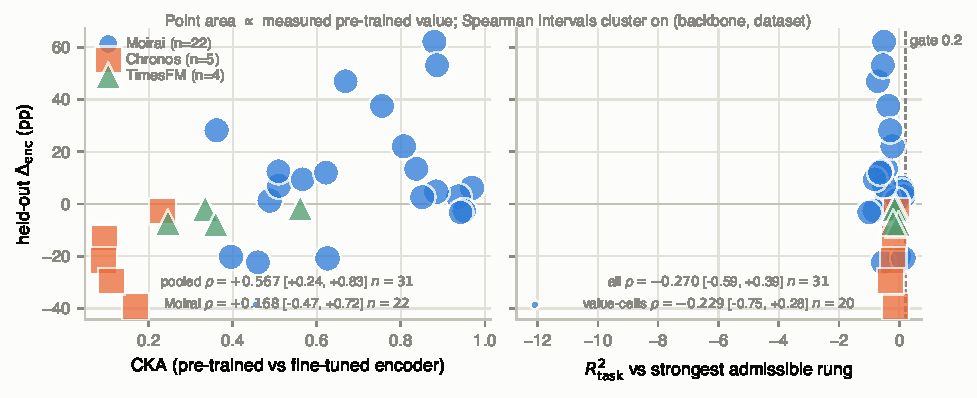
\includegraphics[width=\linewidth]{fig_value_axis.pdf}
\caption{\textbf{Neither drift nor measured pre-trained value orders the encoder
intervention.} Both panels share $y{=}$ held-out $\denc$ (positive $=$ freezing the
encoder did better). Point area is proportional to the graded value score in
\emph{both} panels, so the left panel answers the objection visually: if drift
predicted the outcome wherever there was something to lose, the large points
would trend and the small ones would scatter. Backbone is encoded by colour
\emph{and} marker because CKA is not comparable across architectures, which is why
the pooled left-panel interval must not be read as a within-backbone one. Drawn by
\texttt{paper\_8/fig\_value\_axis.py} from \texttt{results/value\_axis.json}; the
script asserts its own counts against that file and fails rather than drawing a
figure that disagrees with this text.}
\label{fig:valueaxis}
\end{figure}

\begin{table}[!ht]
\centering
\caption{\textbf{The dependence, estimated two ways.} Rank rows are Spearman
$\rho$ with $10{,}000$ bootstrap draws over $(\text{backbone}, \text{dataset})$
clusters, seed~$0$. The slope rows fit all cells at once with backbone identity
absorbed as a fixed effect and both regressors centred, so $b_1$ is the CKA slope
\emph{at mean value}; $b_3$ is the quantity at issue. Emitted by
\texttt{scripts/value\_axis.py --latex}, which delegates the slope fit to
\texttt{scripts/cka\_fixed\_effects.py} rather than refitting it.}
\label{tab:valueaxis}
% GENERATED by scripts/value_axis.py --latex -- do not edit by hand.
\setlength{\tabcolsep}{4pt}
\footnotesize
\begin{tabular}{@{}lrrrl@{}}
\toprule
Relation & $n$ & clusters & $\rho$ or $b$ & 95\% CI over clusters \\
\midrule
CKA vs $\denc$, the value-cells & 20 & 11 & $+0.567$ & $[+0.191, +0.889]$ excludes 0 \\
CKA vs $\denc$, cells with no admissible value & 11 & 7 & $+0.709$ & $[-0.077, +0.901]$ includes 0 \\
CKA vs $\denc$, within Moirai & 22 & 6 & $+0.168$ & $[-0.469, +0.717]$ includes 0 \\
CKA vs $\denc$, pooled (not a licensed reading) & 31 & 15 & $+0.567$ & $[+0.239, +0.828]$ excludes 0 \\
$\Vbest$ vs $\denc$, the value-cells & 20 & 11 & $-0.229$ & $[-0.755, +0.284]$ includes 0 \\
$\Vbest$ vs $\denc$, all cells & 31 & 15 & $-0.270$ & $[-0.592, +0.392]$ includes 0 \\
\midrule
\multicolumn{5}{@{}l}{\emph{Slope scale, all cells at once: $\denc = b_0 + b_1\mathrm{CKA} + \text{backbone FE} + b_2 v + b_3(\mathrm{CKA}{\times}v)$, $v={}$value}} \\
$b_1$, CKA slope at mean value (pp per unit CKA) & 31 & 15 & $+39.8$ & $[-55.1, +179.4]$ includes 0 \\
$b_3$, CKA${\times}$value interaction & 31 & 15 & $-31.5$ & $[-209.6, +166.2]$ includes 0 \\
\bottomrule
\end{tabular}

\end{table}

\textbf{The rank answer: the relation is not stronger where there is more to
lose.}  Restricting to the 20 value-cells gives $\rho{=}{+}0.567$ with clustered
CI $[{+}0.191, {+}0.889]$; the 11 cells with no admissible value give
$\rho{=}{+}0.709$ with CI $[-0.077, {+}0.901]$ (Table~\ref{tab:valueaxis}).  The
restriction the objection asks for does not sharpen the relation, and the
value-cell figure is not evidence that drift orders the outcome: it pools all three
backbones, and within Moirai (the only arm with the cells to ask), the same
statistic is $\rho{=}{+}0.168$ with an interval spanning zero.  We do not test the
difference of those two $\rho$s: a difference of rank statistics on 20 and 11 cells
from 11 and 7 clusters has no usable sampling distribution, and reporting one would
be the kind of number this paper is arguing against.

\textbf{The slope answer, where the dependence is a single coefficient.}  On the
slope scale the interaction is estimable, and it is $b_3{=}{-}31.5$~pp per unit CKA
per unit value with CI $[-209.6, {+}166.2]$, against a CKA slope at mean value of
$+39.8$ with CI $[-55.1, {+}179.4]$.  Two things to say about it and no more.  The
point estimate has the \emph{opposite} sign to the objection (drift orders the
outcome slightly \emph{less} well where there is more value), and the interval
spans zero so widely that only an interaction several times larger than the CKA
slope itself would have been visible at 15 clusters.  \textbf{So this is not a
refutation of the objection; it is the statement that these cells cannot separate
it from no dependence at all.}  That is a weaker claim than we would like to make,
and it is the one the data support.

\textbf{And value does not order the outcome by itself.}  The graded score against
$\denc$ gives $\rho{=}{-}0.270$, CI $[-0.592, {+}0.392]$ across all 31 cells and
$\rho{=}{-}0.229$, CI $[-0.755, {+}0.284]$ across the 20 value-cells, the same
non-result as CKA, on the covariate that was supposed to rescue it.  The right
panel of Figure~\ref{fig:valueaxis} is that row: every point lies left of the
$0.20$ line, and the cells that improve most under encoder adaptation are not the
ones with the least to lose.

% Moved VERBATIM from S6 on 21 Sep 2026 to fund \S\ref{sec:exp4:poscontrol}. It is this appendix's own
% one-sentence summary, which the body restated until now, and it is the paper's ONLY site for the
% claim registered as "cells with nothing to lose" -- hence verbatim rather than reworded. Its closing
% cross-reference pointed here and is dropped; the paragraph now sits in the section it pointed at.
\textbf{Not an artefact of cells with nothing to lose.}  Drift might fail to order
$\denc$ only because 11 of the 31 cells beat no rung of the ladder; grading the
screen rather than dichotomising it says otherwise: the relation is no stronger on
the cells with a measured advantage than on the cells without, and the estimated
interaction has the wrong sign for the objection and an interval far too wide to
settle it.

% ============================================================
\section{Is the Reading Specific to CKA? Six Measures on 59 Encoders}
\label{app:driftmetrics}
% ============================================================

The body reads drift through linear CKA, so a reader is entitled to ask whether
``drift does not order the outcome'' is a fact about representations or a fact
about CKA. Appendix~\ref{app:crosscell} gives the answer that covers the whole
matrix: $\ell_2$ weight drift, a geometrically unrelated quantity defined in
\S\ref{sec:method} alongside CKA, fails on the same 31 cells. This appendix
gives the second answer, on geometry, and states up front what it cannot do.

\textbf{What it cannot do.} Only the $n{=}10$k runs retained encoder
checkpoints. The 22-cell Moirai matrix is $n{=}500/1{,}000$ and kept none, so
this battery \emph{cannot} recompute the within-Moirai $\rho$ under a different
measure; that would require retraining the matrix, on different hardware, which
would perturb every number in the paper. What it can do is test
measure-specificity on the 59 encoders that do exist: Moirai-Small at $h{=}96$,
$n{=}10$k, on ETTh1, ETTh2 and ETTm2, under full fine-tuning and under two
layer-unfreezing regimes (top~3 of~6, and all~6), in seven
(dataset, run-set, regime) groups.

\textbf{Measured on the representations the paper's CKA column describes.} Each
run's record stores \texttt{final\_cka}, computed during training on the first
300 validation evaluation windows with the encoder output mean-pooled. The
battery (\texttt{scripts/drift\_metric\_battery.py}) rebuilds exactly those
windows (extended lookback $96{+}96$, raw values, the model normalising
internally), and recomputes linear CKA as a self-check: it agrees with the
stored value to four decimal places on all 59 encoders, so every other column is
known to describe the same representations rather than a similar-looking set.
The checkpoint load asserts that \texttt{load\_state\_dict(strict=False)}
reports no missing and no unexpected keys, because a namespace mismatch loads
nothing silently and returns CKA ${\approx}1$, which reads as ``no drift''.

\begin{table}[ht]
\centering
\caption{\textbf{Six measures of representation change on 59 Moirai-Small
encoders.} All computed on identical windows and identical pooling. ``$\rho$ with
CKA'' is the rank correlation of each measure with linear CKA over the 59
encoders; the last two columns correlate each measure with forgetting, pooled and
then within each of the six groups of at least five encoders. Forgetting here is
the \emph{selection-split} figure: these runs stored no zero-shot test MSE, so a
held-out contrast cannot be reconstructed from them, and
\S\ref{sec:analysis:heldout} shows same-split scoring can invert the sign of the
intervention. This arm is therefore a comparison of measures, not a held-out
claim. Emitted by \texttt{scripts/drift\_metric\_battery.py}; the pooled column
mixes three datasets and is descriptive for the reason
Appendix~\ref{app:crosscell} gives about pooling.}
\label{tab:driftmetrics}
% GENERATED by scripts/drift_metric_battery.py --report -- do not hand-edit.
\centering
\small
\begin{tabular}{lrrrrrc}
\toprule
 & \multicolumn{3}{c}{over 59 encoders} & & \multicolumn{2}{c}{$\rho$ with forgetting} \\
\cmidrule(lr){2-4}\cmidrule(lr){6-7}
Measure & min & max & mean & $\rho$ with CKA & pooled & per group \\
\midrule
Linear CKA & $+0.194$ & $+0.915$ & $+0.588$ & $+1.000$ & $+0.350$ & $[-0.19,+0.60]$ \\
Linear CKA (token) & $+0.626$ & $+0.957$ & $+0.751$ & $+0.542$ & $-0.123$ & $[-0.33,+0.55]$ \\
RBF CKA & $+0.624$ & $+0.913$ & $+0.734$ & $+0.412$ & $+0.117$ & $[-0.36,+0.90]$ \\
SVCCA & $+0.726$ & $+0.939$ & $+0.776$ & $+0.553$ & $-0.038$ & $[-0.70,+0.35]$ \\
Procrustes sim. & $+0.715$ & $+0.947$ & $+0.818$ & $+0.675$ & $+0.127$ & $[-0.52,+0.80]$ \\
Mean cosine & $+0.660$ & $+0.990$ & $+0.840$ & $+0.073$ & $-0.287$ & $[-0.67,+0.60]$ \\
Eff.\ rank ratio & $+0.969$ & $+1.250$ & $+1.119$ & $-0.251$ & $+0.245$ & $[+0.00,+0.65]$ \\
\bottomrule
\end{tabular}

\end{table}

\textbf{The more invariant the measure, the less drift there is to see.} Linear
CKA spans $0.194$ to $0.915$ across these encoders. SVCCA (invariant to any
invertible linear map, so it asks whether the same information survives in a
possibly rotated and rescaled basis) spans only $0.726$ to $0.939$, and
orthogonal-Procrustes similarity $0.715$ to $0.947$. The cell that CKA scores at
$0.194$ is at $0.73$ on SVCCA. This is the concrete form of the objection
limitation~(7) concedes: a large part of what CKA reports as drift is a change of
basis under which the subspace, and with it the linearly decodable content, is
largely preserved. It is also why we do not claim CKA is invalid (it measures
what it measures), only that a paper cannot infer damage from it.

\textbf{The measures do not order the encoders alike, so ``drift'' is not one
quantity.} Rank correlations among them run from $+0.073$ (linear CKA against
mean cosine, the least invariant measure in the battery) through $+0.412$ (linear
CKA against RBF CKA) to $+0.845$ (RBF CKA against Procrustes). Choosing a
similarity measure chooses an ordering of these encoders. We had expected the
opposite (a family of near-clones), and report the disagreement because it makes
the next paragraph the load-bearing one.

\textbf{No measure orders the outcome either.} Against selection-split
forgetting, the pooled rank correlations run from $+0.350$ (linear CKA) to
$-0.287$ (mean cosine), and the pooled figures are the flattering ones: within
groups, where dataset identity is held fixed, every similarity measure changes
sign across the six groups (linear CKA $[-0.19,{+}0.60]$, RBF CKA
$[-0.36,{+}0.90]$, SVCCA $[-0.70,{+}0.35]$, Procrustes $[-0.52,{+}0.80]$, mean
cosine $[-0.67,{+}0.60]$). Six measures spanning no invariance to full
linear-map invariance therefore reproduce the body's reading rather than
overturning it: the disagreement among them does not resolve into any one of them
ordering the outcome. The single exception is not a similarity measure at all.
The effective-rank ratio (how many directions the representation uses after
fine-tuning against before) is above $1$ on 55 of the 59 encoders
($0.969$--$1.250$, so fine-tuning generally \emph{expands} the spectrum) and is
the one column with no negative group value ($[+0.00,{+}0.65]$). At six groups,
one backbone and one sample size we record that as a lead for future work, not a
diagnostic; it is exactly the kind of pattern this paper's own prospective test
(\S\ref{sec:analysis:prospective}) was built to keep us honest about.

% Round 10 (A2). A reviewer asked for the paper's claim to be stated at the level of the METRIC FAMILY
% rather than of linear CKA alone, which is the generalisation this appendix's evidence supports and the
% body's does not. It is stated HERE, next to that evidence and inside the page-exempt appendix, rather
% than in \S6: the body has no free lines this round, and a generalisation printed a page away from the
% five intervals that license it would be the kind of claim this paper's own audit trail keeps catching.
% THE SCOPE CLAUSE IS NOT OPTIONAL. These 59 encoders are one backbone, one capacity, one horizon and
% one sample size; they contain NONE of the paper's 31 $\denc$ cells; and their outcome column is
% single-arm selection-split forgetting, not the intervention contrast. So the sentence is a reading of
% this arm, hedged in both directions, and the body's claim stays where the intervention is.
\textbf{What this licenses, and what it does not.} Read together, the six
measures support the generalisation our title implies but the body does not
claim: on this arm, \emph{post-fine-tuning representation similarity should not
be assumed to identify harmful encoder adaptation}, whichever similarity is
chosen. What that reading cannot be is a claim about $\denc$: these 59 encoders
are one backbone at one capacity, horizon and sample size, none of them among the
31 cells the intervention is measured on, and their outcome column is
single-arm selection-split forgetting. A measure that failed here could still
order a held-out intervention elsewhere, and we did not test one that does.

% ============================================================
\section{What Predicts the Intervention, and Why None of It Is a Shortcut}
\label{app:predictor}
% ============================================================

If some quantity measurable from one run ordered B$-$D, a practitioner could
skip the frozen control. We tested every candidate we had, within Moirai only,
because it is the only arm with enough cells to ask (22). The statistic is again
Spearman $\rho$ against held-out B$-$D with a $10{,}000$-resample bootstrap CI at
both resampling levels, from \texttt{scripts/clustered\_inference.py}:

% GENERATED by scripts/clustered_inference.py --latex -- do not edit by hand.
\begin{center}\small
\setlength{\tabcolsep}{4pt}
\begin{tabular}{@{}lcccll@{}}
\toprule
Predictor (Moirai only) & $n$ & Cl. & $\rho$ & 95\% CI over cells & 95\% CI over clusters \\
\midrule
forg$_\text{B}$ (condition~B only) & 22 & 6 & $+0.894$ & $[+0.667, +0.981]$ excludes 0 & $[+0.594, +0.965]$ excludes 0 \\
forg$_\text{D}$ & 22 & 6 & $+0.073$ & $[-0.324, +0.429]$ includes 0 & $[-0.343, +0.412]$ includes 0 \\
Gate $\Vb{\text{ridge}}$ & 22 & 6 & $-0.293$ & $[-0.706, +0.188]$ includes 0 & $[-0.712, +0.709]$ includes 0 \\
CKA & 22 & 6 & $+0.168$ & $[-0.328, +0.598]$ includes 0 & $[-0.469, +0.717]$ includes 0 \\
$\ell_2$ weight drift & 21 & 5 & $+0.318$ & $[-0.122, +0.673]$ includes 0 & $[-0.329, +0.861]$ includes 0 \\
\bottomrule
\end{tabular}
\end{center}


\noindent Weight drift covers 21 of the 22 cells because ILI's run records
retain no drift measurement. The gate row is the same figure reported in
Appendix~\ref{app:gatecorrection}; it appears here beside its competitors. \textbf{These 22 cells come from six
clusters}, and the gate row is the one place in the paper where that distinction
changes a verdict: see Appendix~\ref{app:clustered}.

\textbf{The forg$_\text{B}$ result is an identity, not a discovery.} B$-$D
$\equiv$ forg$_\text{B} - \text{forg}_\text{D}$ holds \emph{exactly}, because
both terms are percentage changes against the same zero-shot reference: over all
cells the maximum deviation is
$\max|(\text{forg}_\text{B}-\text{forg}_\text{D})-(\text{B}{-}\text{D})|
= 0.000$. The dispersion is then overwhelmingly on the B side, SD $26.2$ against
forg$_\text{D}$'s $8.1$, so B$-$D is close to a rescaled copy of
forg$_\text{B}$ and $\rho{=}{+}0.894$ is close to arithmetic rather than to a
finding. It confers no ability to skip condition~D: forg$_\text{B}$ exists only
once condition~B has been run, and at that point running D is one further run on
the same cell. This is exactly the kind of correlation that looks like a
shortcut and is not, and the near-zero forg$_\text{D}$ row is the reason: the
rule works only because the frozen arm happens to be nearly constant on this
backbone, which is an empirical property of these cells and not a theorem.

% Figure 1's panel (b) plotted this axis until 20 Sep 2026, when the main figure went back to CKA
% because the title states the CKA-to-outcome relation as the finding. The gate-to-outcome relation is
% a different claim and is unchanged, so the scatter moves here rather than being deleted -- and here
% it can carry the ILI cell, which the panel's xlim silently clipped for two rounds.
\begin{figure}[t]
\centering
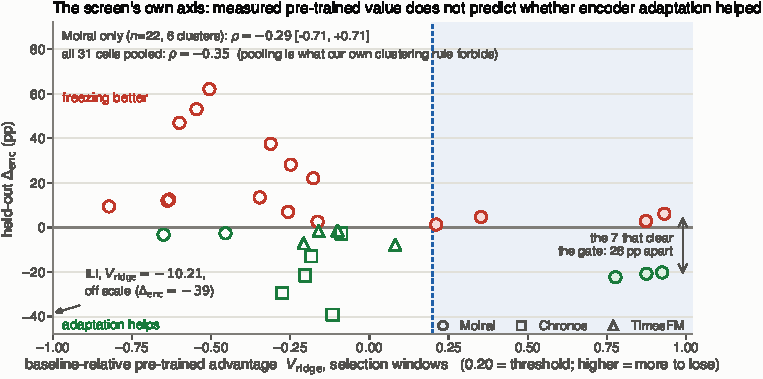
\includegraphics[width=\linewidth]{figA_gate_scatter.pdf}
\caption{\textbf{The screen's own axis.} All 31 intervention cells as the
selection-split gate against held-out $\denc$ (positive ${=}$ freezing better).
Filled markers clear $\Vb{\text{ridge}}{\geq}0.20$; the shaded strip is the only
region a cell could occupy and still satisfy clause~(i) of the degradation
definition, and most of the cells in it lie \emph{below} zero, where letting the
encoder adapt helped.  The two axes are scored on disjoint window sets, so a cell's
horizontal position is not a re-description of its vertical one.  ILI is named on the
frame rather than plotted: its gate is $-10.21$, and an axis wide enough to include
it compresses the other 30 cells into a fifth of the panel.}
\label{fig:gatescatter}
\end{figure}

\textbf{The gate's continuous score points the wrong way, but only the sign is
supported} (Figure~\ref{fig:gatescatter}). On the same 22 cells the gate correlates \emph{negatively} with
held-out B$-$D, $\rho{=}{-}0.293$ on the selection-split gate this paper reports
as primary. Neither resampling level supports an interval claim: cells give
$[-0.706, +0.188]$ and the six clusters give $[-0.712, +0.709]$. On the
retrospective test-side gate the same correlation is $\rho{=}{-}0.518$ with a
cell-level CI of $[-0.840, -0.040]$ that \emph{does} exclude zero, and a clustered
CI of $[-0.810, +0.500]$ that does not, so we do not read it as excluding zero
(Appendix~\ref{app:clustered}); scoring the gate on the split that does not touch
the outcome removes it independently, and the magnitude nearly halves between the two splits, which is
itself the point of \S\ref{sec:analysis:prospective}, that there is no stable
ordering here to exploit. The
mechanism is legible in Table~\ref{tab:heldout_all}: the cells with the largest
measured pre-trained advantage are the Moirai/ETTh2 cells, and three of those
five are the cells where full fine-tuning beats the frozen encoder by the most
(B$-$D $-20.2$ to $-22.3$~pp), while the cells with the most negative
gates (Weather and ETTh1) are where freezing wins by tens of points, up to
$+62.1$~pp. A practitioner following ``preserve where the gate fires'' would
therefore freeze precisely where adapting the encoder pays best. We report this
at the strength it has: a within-Moirai point estimate on 22 retrospective cells
from six series, with a clustered interval that spans zero. \textbf{The negative
sign is a description of these cells, not an interval-supported claim, and the
magnitude is not estimated to any useful precision.} The mechanism above is
legible cell by cell in Table~\ref{tab:heldout_all} and does not depend on the
correlation surviving; that is why we still report the direction.

\textbf{The other two arms cannot adjudicate.} On TimesFM ($n{=}4$) the gate
gives $\rho{=}{+}0.800$, CI $[+0.333, +1.000]$, forg$_\text{B}$ gives
$+1.000$ and CKA $+0.400$, CI $[-0.778, +1.000]$; on Chronos ($n{=}5$) the gate
gives $\rho{=}{+}0.500$, CI $[-0.667, +1.000]$, and forg$_\text{B}$ gives
$-0.100$. These are reported for completeness and are uninformative at four and
five cells: a bootstrap over four cells resamples only a few distinct rank
patterns, so even the TimesFM gate interval, which nominally excludes zero, is
an artefact of that granularity and we read nothing from it. Chronos's
forg$_\text{B}$ carries a further defect and is flagged
\texttt{forg\_confounded} in the code: a head/decoder mismatch means its B-side
number is not a clean per-condition forgetting measurement, so it is retained
only to show where the forg$_\text{B}$ rule breaks and is never quoted as a
forgetting value.

\textbf{Nothing here is a replacement diagnostic.} The honest summary of this
appendix and of Appendix~\ref{app:crosscell} together is that no observational
quantity we measured orders the intervention in a usable direction: CKA and
$\ell_2$ drift do not order it, the gate orders it \emph{backwards}, and the one
predictor that tracks it does so by identity and only after the run that would
have told you the answer anyway. On the evidence in Table~\ref{tab:heldout_all},
the only reliable way to know whether encoder adaptation helped a given cell is
to run both conditions on that cell.

% ============================================================
\section{The Same Cells Priced as a Decision, Post-Hoc}
\label{app:decision}

Every result above is a statement about an interval: a within-Moirai slope whose
sign is not resolved, a $\Delta R^2$ that is negative but whose dispersion cannot be
quoted.  A reader may fairly reply that none of that is evidence \emph{against} a
relationship.  So this subsection asks the question in the units a practitioner
would act in, where the claim is falsifiable rather than merely unproven: what would
following a CKA rule have been \emph{worth}?  \textbf{This analysis is post-hoc.}
Unlike Table~\ref{tab:cka_loco} nothing here was registered in advance; the policy
family, the objective and the folds were all chosen after the outcomes were known,
and the emitter (\texttt{scripts/cka\_decision\_value.py}) says so in its first
paragraph.

\textbf{The construction.}  A practitioner facing one cell picks full fine-tuning or
a frozen encoder, and collects $\denc$ on every cell they freeze, so the realised
saving of a policy against the default of always adapting is the mean over all 31
cells of $\denc \cdot \mathbf{1}[\text{freeze}]$, in percentage points of MSE.
Every single-threshold CKA rule lies in one family, which puts six policies on one
scale (Table~\ref{tab:cka_decision}).  \textbf{The out-of-sample row is the only one
a practitioner could have followed}: the cut \emph{and} its orientation are searched
on the 14 training clusters and applied unchanged to the held-out cluster, so every
cell's decision is taken without seeing that cell.  Candidate cuts are interior, so
the search cannot quietly return \emph{always freeze} and have it counted as CKA
informing anything; both degenerate policies are priced as rows of their own.

% The result that does NOT go this paper's way is stated first and in its own bold sentence, rather
% than after the two that do. It would be cheap to lead on the prescribed-orientation row (which is
% strongly against the shortcut) and leave +7.47 to the table; the reviewer's objection is precisely
% that the paper argues its null too hard, and burying the one number that cuts the other way is what
% arguing too hard looks like.
\textbf{The number that does not favour our claim, first.}  The best-orientation
rule is worth $+7.47$~pp out of sample -- not zero, and not what a reader would
predict from a headline that drift carries no actionable information.  Two things
bound it.  Its interval is $[-4, +16]$~pp and it is worth nothing or less in $25\%$
of cluster-bootstrap draws, so these cells do not \emph{establish} a saving at all:
this is a policy whose value is unresolved, exactly as the slope's sign is
unresolved, and the honest reading is the same in both cases.  And the orientation
that earns it is \textbf{the inverse of the one the literature prescribes}: it
freezes the cells whose representations moved \emph{least}.  Freezing where drift is
largest -- what forgetting mitigation actually recommends -- is worth $-6.97$~pp
$[-10, +14]$, and is worth nothing or less in $80\%$ of draws.  A practitioner who
followed the prescription on these cells would have lost about seven points of MSE
per cell relative to not measuring drift at all.

\textbf{What the other rows add.}  Always freezing, ignoring CKA entirely, is worth
$+2.91$~pp $[-13, +15]$, so the best-orientation rule's advantage over the cheap
policy that reads no representation at all is $+4.56$~pp, nothing or less in $20\%$
of draws.  Choosing the cut on the cells it is then scored on pays $+8.57$~pp: the
$+1.10$~pp gap $[0, +13]$ is the price of a retrospectively chosen threshold, and it
is what \S\ref{sec:conclusion}'s ``chosen on those same cells, so a lower bound and
not a validated classifier'' costs, measured.  Per-cell hindsight is worth
$+10.38$~pp $[+1, +19]$.  Out of sample the rule freezes 16 of the 31 cells and puts
8 of them on the wrong side of its own decision, against 5 for the in-sample cut --
the same count Figure~\ref{fig:screen}b reports for the best threshold, reached
here by maximising saving rather than by minimising misplacement, which are
different objectives that happen to agree on this data.

\textbf{What we take from it, and what we do not.}  We do not claim this refutes a
CKA rule: a point estimate of $+7.47$~pp is not a refutation, and one policy family
on 15 clusters cannot speak for a per-backbone cut, a multivariate rule or a
continuous-shrinkage policy.  What it supports is narrower and is the claim this
paper makes: on these cells the evidence does not establish a saving stable enough
to act on, and the direction in which acting would have paid is the opposite of the
direction the mitigation literature points.  Both readings survive the reviewer's
objection to the null, because neither of them is the assertion that no relationship
exists.

% tables/cka_decision.tex carries its own table environment, caption and label.
% GENERATED by scripts/cka_decision_value.py --json --latex -- do not edit by hand.
\begin{table}[t]
\centering
\caption{\textbf{What would acting on CKA have saved?} The same
31 cells read as a decision rather than a correlation. A practitioner
choosing per cell between full fine-tuning and a frozen encoder collects
$\denc$ (positive ${=}$ freezing better) on every cell they freeze, so
\emph{saving} $=$ mean over all 31 cells of
$\denc \cdot \mathbf{1}[\text{policy freezes}]$, in percentage points of MSE,
against the default of always adapting. \textbf{The out-of-sample row is the only
one a practitioner could have followed}: the threshold and its orientation are
searched on the 14 training clusters and applied unchanged to the
held-out cluster, so each cell's decision is made without seeing it. The row below
it is the same search run on all cells at once, and the difference between them,
$+1.10$~pp $[0, +13]$,
prices the optimism in a retrospectively chosen cut.
\textbf{The headline is the interval, not the point estimate}: the best-orientation
rule's $+7.47$~pp comes with
$[-4, +16]$ and is ${\leq}0$ in
25\% of draws, so it is a
policy whose value these cells cannot establish, not one they refute.
\textbf{And the orientation that earns it is the inverse of the prescribed one}:
freezing where drift is \emph{largest} -- what forgetting mitigation actually
recommends -- is worth $-6.97$~pp
$[-10, +14]$, and the row above it buys its point
estimate by freezing the cells that moved \emph{least}, a direction available only
because we searched both. That rule still puts
8 of the 31 cells on the wrong side of
its own decision out of sample (16 of them wanted
freezing), against 5 for the in-sample cut.
\textbf{This analysis is post-hoc and descriptive}: unlike
Table~\ref{tab:cka_loco}, nothing here was pre-registered, and the family searched
is a single global CKA threshold in either orientation -- a per-backbone or
multivariate rule could do better, and 15 clusters cannot rule that out.
Candidate cuts are interior (midpoints between consecutive distinct CKA values), so
the search cannot return \emph{always freeze} or \emph{always adapt} and have it
counted as CKA informing the decision; both are priced as rows of their own.
Intervals are 95\% percentile cluster bootstrap
(10,000/10,000 draws kept, a draw discarded when it leaves
fewer than three distinct clusters), re-running the whole
leave-one-cluster-out procedure inside each draw with duplicated clusters sharing one
fold id. Every statistic is a mean of bounded per-cell quantities, so unlike
$\Delta R^2$ in Table~\ref{tab:cka_loco} these percentiles are reproducible --
\textbf{to whole percentage points, which is why they are quoted that way}: at two
decimals the bounds move across bootstrap seeds (this table's headline lower bound
came out $-3.97$, $-3.61$, $-3.68$ and $-3.67$ on seeds 0, 1, 7 and 13), and
\texttt{-{}-seedcheck} checks every figure quoted here at its printed precision.
The point estimates and the misplacement counts carry no seed at all.}
\label{tab:cka_decision}
\small
\begin{tabular}{lrr}
\toprule
Policy & Saving (pp) & 95\% cluster CI \\
\midrule
Always adapt (fine-tune everything) \emph{-- the baseline} & $0.00$ & \emph{by construction} \\
Always freeze the encoder, ignoring CKA & $+2.91$ & $[-13, +15]$ \\
CKA rule \emph{as prescribed}: freeze where drift is largest & $-6.97$ & $[-10, +14]$ \\
\textbf{CKA threshold, best orientation, chosen out of sample} & $+7.47$ & $[-4, +16]$ \\
\quad the same rule, threshold chosen on the cells it is scored on & $+8.57$ & $[0, +18]$ \\
Oracle: freeze exactly the cells that wanted it & $+10.38$ & $[+1, +19]$ \\
\bottomrule
\end{tabular}
\end{table}


% ============================================================